\newpage

\titleformat % design des titres des chapitres
{\chapter}
[display]
{\centering\normalfont\Large\scshape\bfseries}
{\rule[3pt]{0.15\linewidth}{3pt}\quad\chaptertitlename~\thechapter\quad \rule[3pt] {0.15\linewidth}{3pt}}
{0\baselineskip}%espace vertical entre chapitre et nom du chapitre
{\rule{\linewidth}{0.5pt}\break\Huge}
[\vspace{-0.5\baselineskip}\rule{\linewidth}{0.5pt}\vspace{0\baselineskip}]

\let\clearpage\relax% Stop LaTeX from going to a new page; and
\vspace*{5.5cm}%

\chapter{Réalisation du projet}
Dans ce chapitre, je vais présenter la réalisation du projet. D’abord je vais exposer
les interfaces de l’application, puis nous décrirons les différentes fonctionnalités de ces dernières.

\newpage

\section{Interface d'acceuil}

\begin{figure}[!h]
    \centering
    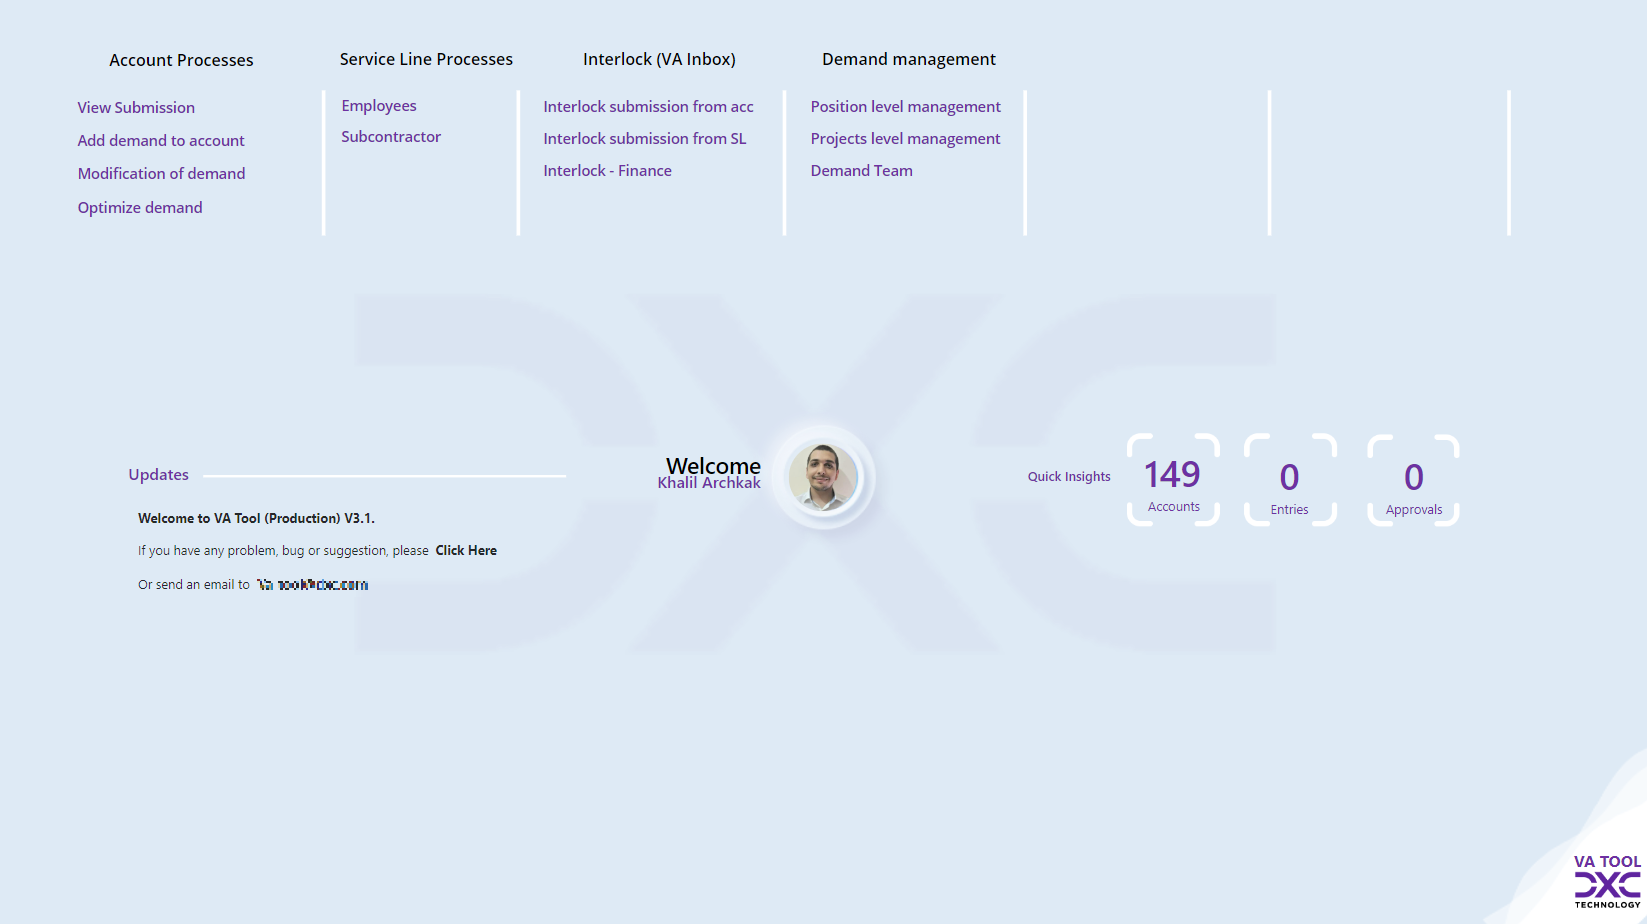
\includegraphics[scale=0.4,keepaspectratio]{Rapport de stage PFE chez DXC/figures/Home_Page.png}
    \caption{Interface d'accueil}
\end{figure}

La page d'accueil regroupe les différentes procédures possibles que propose l'application dans un menu verticale à savoir les procédures en relation avec les comptes, le service line, l'interlock de ces deux dernier mais aussi la gestion des demandes.
\\[0.1cm]

Commençons par donner une explication générale à chacune des sections présente dans le menu de la page d’accueil :
\\

\begin{itemize}
    %% ======================== Account Processes ===============================
    \item[\ding{118}] \textbf{Account Processes:}
    
        \vspace{0.5cm}
        %% ====================== Add demand to account ==============================
        \begin{itemize}
            \item[\textbullet] \textbf{Add demand to account:} Cette option permet à un administrateur de compte de faire une demande d'ajout de masse salariale à son compte, les demande d'ajout sont divisé en quatre parties :
            
            \begin{itemize}
                \item[\ding{51}] \textbf{Existing Account:} est utiliser pour ajouter une demande pour un client existant.
                \item[\ding{51}] \textbf{New Logo:} est utiliser pour ajouter une demande pour un futur client.
                \item[\ding{51}] \textbf{Roll-Off/Roll-On:} est utiliser lorsqu’un employé change de projet mais reste avec le même  compte. 
                \item[\ding{51}] \textbf{Placeholder - Add demand:} joue le rôle d'une entrée temporaire pour un futur besoin, cette dernière peut être convertit en une entrée VA dans le futur.
            \end{itemize} 
            
            %% ====================== Modification of demand ==============================
            \newpage
            \item[\textbullet] \textbf{Modification of demand:} Cette option permet a un administrateur de compte de modifier les information d'une position ou bien employé: 
            
            \begin{itemize}
                \item[\ding{51}] \textbf{Modification of demand:} qui est composé de deux lever a savoir Run-Off qui represente un employé dont le contrat arrive à son terme ou bien extension qui va permettre a l'administrateur du compte d'étendre sont contrat.
                \item[\ding{51}] \textbf{Placeholder Modification:} of demand qui est similaire au placeholder add demand expliqué precedement, cette dernière permet de préparer une entrée de modification pour un futur besoin, elle aussi peut être convertit en une entrée VA dans le futur.
            \end{itemize}
            
            \vspace{0.5cm}
            %% ====================== Optimize demand ==============================
            \item[\textbullet] \textbf{Optimize demand:} Cette option permet à un administrateur de compte comme son nom l'indique d'optimiser sa demande en effectuant une opération de work migration ou bien Productivity :
            
            \begin{itemize}
                \item[\ding{51}] \textbf{Work Migration/LPI:} est utilisé lorsequ'on veut migrer un employé vers un autre centre de delivery DXC.
                \item[\ding{51}] \textbf{Productivity:} Est utilisé lors d'un gain au niveau du coup de l'employé, par exemple en cas ou le remplacement d'une position nous coute moins chère.
            \end{itemize}
            
            \vspace{0.5cm}
            %% ====================== View submissions ==============================
            \item[\textbullet] \textbf{View submission :} Cette option permet à un administrateur de compte de voir ces entrées, de les modifier, d'annuler une entré, de créer à partir d'une entrée VA une entrée DCT mais aussi de dupliquer son entrée.
            
        \end{itemize}
        
    \vspace{0.5cm}
    
    %% ======================== Service Line Processes ===============================
    
    \item[\ding{118}] \textbf{Service Line Processes} 
        
        \vspace{0.5cm}
        
        \begin{itemize}
        
            %% ======================== SL Employees ===============================
            \item[\textbullet] \textbf{Employees:} Cette option permet au responsable du service line d'effectuer différente demande sur les employés à savoir : 
            \begin{itemize}
                \item[\ding{51}] \textbf{Modification of demand:} De la même manière qu'un administrateur de compte un responsable de service line peut effectuer une opération de run-off ou bien extension sur l'un des employés.
                \item[\ding{51}] \textbf{Work migration/LPI:} Il peut aussi effectuer une action de migration sur l'un des employés.
                \item[\ding{51}] \textbf{Productivity} Il peut également réaliser une modification de type productivity sur l'un des employés.
                \item[\ding{51}] \textbf{View submission :} Il dispose aussi d'une interface dans laquelle il peut parcourir ces différentes entrées, les modifier ou bien dupliquer.
            \end{itemize} 
            
            \vspace{0.5cm}
            
            %% ======================== Subcontractors ===============================
            
            \item[\textbullet] \textbf{Subcontractors :} Cette option est resérvé au subcontractors, les subcontractors sont les centre de delivery qui ne sont pas a 100\% DXC, Par exemple DXC technology Maroc est une jointure entre la CDG (49\%) et DXC technoloty (51\%) ce qui fait d'elle un subcontractor.
            Pour l'instant le design des differentes opération de cette option est toujours en discussion.
            
        \end{itemize}
        
   
    \newpage
    %% =========================== Interlock Process =============================
    \item[\ding{118}] \textbf{Interlock Process}
    
    \vspace{0.5cm}
    
        \begin{itemize}
        
            %% ======================== Interlock from Account ===============================
            \item[\textbullet] \textbf{Interlock Submission from Account:} Cette option permet au responsable de service line de confirmer l’information saisit par les responsables du compte mais aussi ajouter d'autre information et ensuite approuver la soumission.
            
            \vspace{0.5cm}
            
            %% ======================== Interlock from SL ===============================
            \item[\textbullet] \textbf{Interlock Submission from Service Line:} Cette option permet au responsable des compte de confirmer l’information saisit par les responsables du service line mais aussi ajouter d'autre information et ensuite approuver la soumission.
            
            \vspace{0.5cm}
            
            %% ======================== Interlock from Finance ===============================
            
            \item[\textbullet] \textbf{Interlock Submission from Service Line:} Cette option permet au responsable de la finance de confirmer eux aussi les entrées de ces deux derniers, Pour l'instant le processus est toujours en cours de discussion.

        \end{itemize}
    
    %% =========================== Demand Management =============================
    
    \vspace{0.5cm}
    
    \item[\ding{118}] \textbf{Demand Management}
    
    \vspace{0.5cm}
    
        \begin{itemize}
            
            %% ====================== Position Level Management ========================
            \item[\textbullet] \textbf{Position level management:} Cette interface est consacrée à la saisie de demande par les comptes dans un format DCT.
                
                \begin{itemize}
                    \item[\ding{51}] \textbf{Create demand:} Pour créer une nouvelle demande.
                    \item[\ding{51}] \textbf{Update demand:} Pour modifier une demande existante.
                    \item[\ding{51}] \textbf{View submission} Une interface qui permet à l'utilisateur de voir ces différentes soumissions de les modifier, de consulter les commentaires de la part de l'examinateur de la demande, d'attacher un fichier pièce jointe d'approbation, de dupliquer une demande, mais aussi de l'annuler.
                \end{itemize}
                
            \vspace{0.5cm}
            
            %% =========================== Project  Level Management ==============================
            
            \item[\textbullet] \textbf{Project level management:} Cette interface est consacrée à la saisie de nouveau project.
            
                \begin{itemize}
                        \item[\ding{51}] \textbf{Create a new project:} Pour créer un nouveau projet.
                        \item[\ding{51}] \textbf{Update an existing project:} Pour modifier un projet existant.
                        \item[\ding{51}] \textbf{Close an existing project:} Pour fermer un projet existant.
                        \item[\ding{51}] \textbf{View submission} Cette interface permet à l'utilisateur de voir ces différentes soumissions.
                \end{itemize}
            
            %% ================================ Demand team ====================================
            
            \vspace{0.5cm}
            
            \item[\textbullet] \textbf{Demand team :} Cette interface est consacrée aux experts qui vont examiner les différentes demandes pour les valider.
            
             \begin{itemize}
                        \item[\ding{51}] \textbf{Demand validation check:} Cette interface contient la liste de toutes les entrées soumises par les comptes, l'examinateur en cliquant sur une entrée peut l'assigner à lui-même et ensuite effectuer les différentes vérifications, par la suite il peut la valider.
                        \item[\ding{51}] \textbf{DCT position export:} Après avoir valider une soumission DCT l'examinateur peut ensuite accéder à cette interface qui va lui permettre d'exporter toutes les soumissions validées pour les ajouter à l'outil corporel de DXC qui gère toutes les demandes.
                \end{itemize}
            
        \end{itemize}
    
\end{itemize}

La page d'accueil contient aussi un aperçu rapide du nombre de compte affecté pour l'utilisateur, le nombre d'entré saisie par l'utilisateur.
\\[0.3cm]
On peut aussi être renvoyer vers une autre application qui nous permet d'enregistrer les différentes suggestions des utilisateurs ou bien envoyer un email en cas de problème à la mailbox de support.

%Add demand to account
\section{Compte - Ajout de masse salariale}


% ========================= Existing account =================================
\subsection{Compte existant}

\subsubsection{Présentation de l'interface :}

L'interface suivante permet a un responsable de compte de faire une demande d'ajout, c'est a dire ajouter une position pour une opportunité ou bien projet.


\subsubsection{Regle de gestion:}

Le tableau suivant represente les different regle de gestion que l'interface doit respecter :

\vspace{0.2cm}

\tikzset{ 
    table/.style={
        matrix of nodes,
        row sep=-\pgflinewidth,
        column sep=-\pgflinewidth,
        nodes={
            rectangle,
            draw=black
        },
        minimum height=1.5em,
        text depth=0.5ex,
        text height=2ex,
        nodes in empty cells,
%%
        every even row/.style={
            nodes={fill=gray!70}
        },
        column 1/.style={
            nodes={text width=10em,align=center}
        },
        column 2/.style={
            nodes={text width=24em}
        },
        column 3/.style={
            nodes={text width=5em,align=center}
        },
        row 1/.style={
            nodes={
                font=\bfseries,
                align=center,
                fill=black,
                text=white,
            }
        },
        row 2/.style={
            nodes={
                fill=black,
                text=white,
                text depth=4ex,
            }
        },
        row 3/.style={
            nodes={
                fill=white,
                text=black,
                text depth=4ex,
            }
        },
        row 4/.style={
            nodes={
                fill=black,
                text=white,
                text depth=4ex,
            }
        },
        row 5/.style={
            nodes={
                fill=white,
                text=black,
                text depth=4ex,
            }
        },
        row 6/.style={
            nodes={
                fill=black,
                text=white,,
                text depth=11ex,
            }
        },
        row 7/.style={
            nodes={
                fill=white,
                text=black,
                text depth=7ex,
            }
        }
    }
}

\begin{tikzpicture}

\matrix (first) [table,text width=6em]
{
 Regle de gestion  & Description & Type \\
 RG01 & Toutes les informations de l’étape 2 doivent être remplis & Métier \\
 RG02 & Si une information de l'étape 2 ou bien 1 est vide le bouton de soumission doit être désactiver. & Métier \\
 RG03 & La valeur du FTE doit etre entre 0 et 1 & Métier \\
 RG04  & Le champ monthly cost n'accepte que des chiffres & Métier \\
 RG05  & Si l'utilsateur selectionne "Yes" dans le champ "in account forcast", Il doit imperativement remplire les deux champ suivant a savoir le l'année fiscale et le mois. & Métier \\
 RG06  & Une fois l'entrée soumis tout les champs doivent etre réinitialiser puis envoyer l'utilisateur a l'interface "view submission" & IHM\\
};


\end{tikzpicture}


\newpage

\subsubsection{Fonctionnement de l'interface :}

La figure ci-dessous représente l'interface qui permet de faire une demande de croissance par un administrateur de compte :

\begin{figure}[!h]
    \centering
    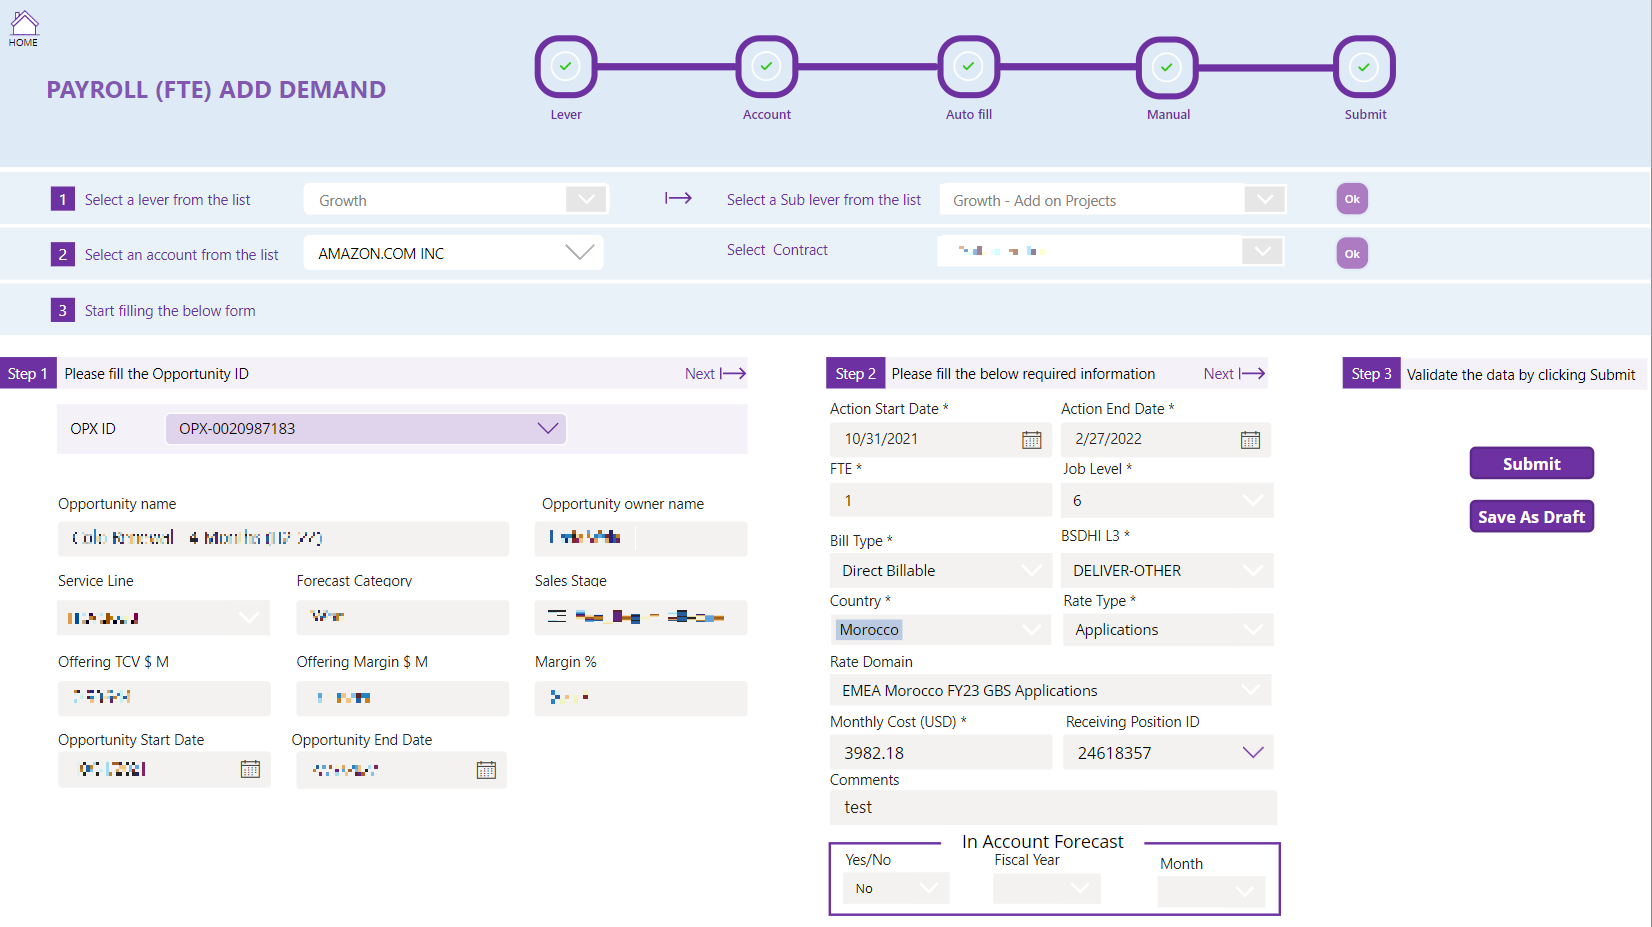
\includegraphics[scale=0.4,keepaspectratio]{Rapport de stage PFE chez DXC/figures/existin_account.png}
    \caption{Ajout de demande - Compte existant}
\end{figure}

La procédure pour saisir une entrée de type croissance est la suivante :

\begin{enumerate}
    
    \item L'utilisateur commence par sélectionner le sub-lever, qui représente la catégorie de la demande d'ajout pour un projet ou bien une croissance stratégique ou autres ensuite il doit cliquer sur le bouton ok.
    \vspace{0.1cm}
    \item Ensuite l'utilisateur doit sélectionner le compte et le contrat qu'il souhaite.
    \vspace{0.1cm}
    \item Puis apparait diffèrent champ qu'il doit remplir, pour l'étape 1 il suffit de sélectionner un OPX-ID qui représente un identificateur d'une opportunité ensuite toutes les informations sont automatiquement remplis.
    \vspace{0.1cm}
    \item La deuxième étape est saisie par l'utilisateur il doit remplir toutes les informations de la demande
    \vspace{0.1cm}
    \item Finalement l'utilisateur a deux choix soit soumettre directement ou bien la soumettre en tant que brouillon s'il n'est pas sur ou souhaite changer les informations de l'entrée dans le futur

\end{enumerate}

\newpage

% =========================== New logo =================================

\subsection{New Logo}

\subsubsection{Présentation de l'interface :}

L'interface suivante permet à un responsable de compte de faire une demande d'ajout de la même manière que la précédente la seule différence est l'utilisation du contrat Salesforce a la place du nom du compte.

\subsubsection{Regle de gestion:}

L'interface doit respecter le même tableau de règle de gestion vu précédemment.

\subsubsection{Fonctionnement de l'interface :}

\begin{figure}[H]
    \centering
    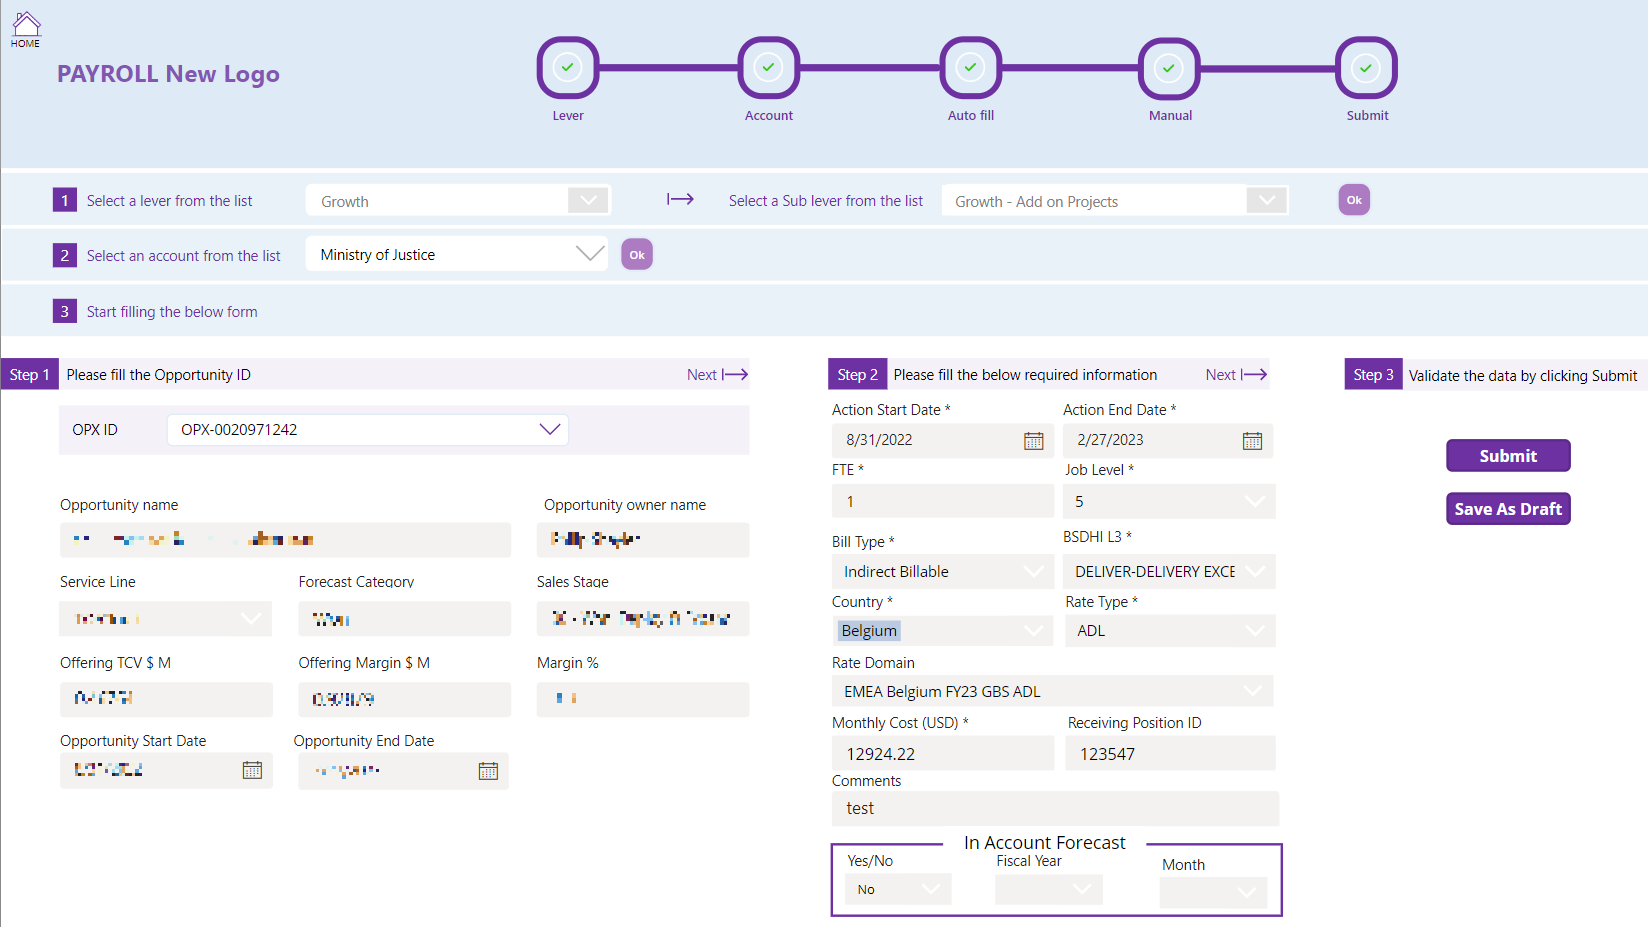
\includegraphics[scale=0.4,keepaspectratio]{Rapport de stage PFE chez DXC/figures/New_Logo.png}
    \caption{Ajout de demande - New Logo}
\end{figure}

Ce formulaire fonctionne de la même façon que le précèdent la seule différence est dans le choix du compte, dans ce dernier le choix du compte est fait à travers le contrat Salesforce car le compte n'est pas encore dans la base de données financière de DXC d'où la nomination "New Logo".

\newpage

% =========================== Roll-Off / Roll-On =================================

\subsection{Roll-Off / Roll-On}

\subsubsection{Présentation de l'interface :}

L’interface suivante permet à un responsable de compte de faire une demande d’ajout, la différence est que dans ce cas un employé va changer de projet mais va rester avec le même compte.

\subsubsection{Regle de gestion:}

L’interface doit respecter le même tableau de règle de gestion vu précédemment.

\subsubsection{Fonctionnement de l'interface :}

\begin{figure}[H]
    \centering
    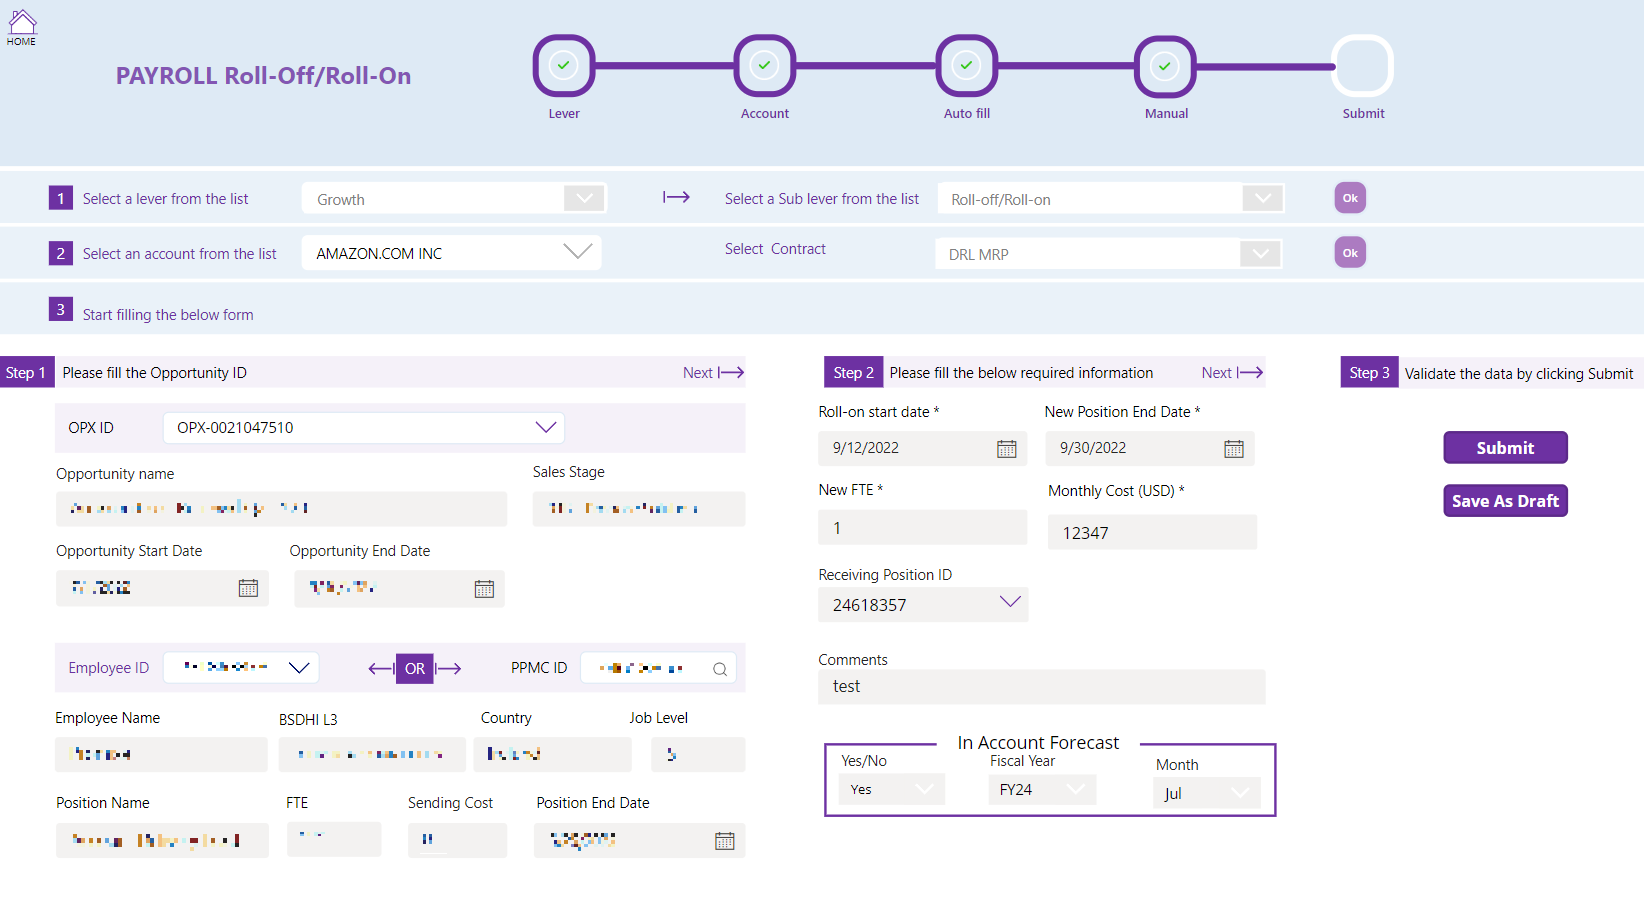
\includegraphics[scale=0.4,keepaspectratio]{Rapport de stage PFE chez DXC/figures/rolloff_rollon.png}
    \caption{Ajout de demande - Roll-Off / Roll-On}
\end{figure}

La procédure pour saisir une entrée de type Roll-Off/Roll-On est la suivante :

\begin{enumerate}
    
    \item L'utilisateur doit sélectionner le compte et le contrat qu'il souhaite.
    \vspace{0.1cm}
    \item L'étape 1 est divisé en deux, La première partie est utilisé pour collecter les informations en relation avec la nouvelle opportunité, la deuxième partie est utilisée pour assembler les informations en relation avec l'employé.
    \vspace{0.1cm}
    \item La deuxième étape est saisie par l'utilisateur il doit remplir toutes les informations pour compléter l'entrée.
    \vspace{0.1cm}
    \item Finalement l'utilisateur a deux choix soit soumettre directement ou bien la soumettre en tant que brouillon s'il n'est pas sur ou souhaite changer les informations de l'entrée dans le futur

\end{enumerate}

% =========================== PlaceHolder - Add Demand =================================

\subsection{PlaceHolder - Add Demand}

\subsubsection{Présentation de l'interface :}

L’interface suivante permet à un responsable de compte de créer une sorte de demande temporaire, c'est à dire ici l'utilisateur peut créer une demande de croissance avec un FTE supérieur à 1, ensuite la convertir en plusieurs entrée VA.

\subsubsection{Regle de gestion:}

Le tableau suivant represente les different regle de gestion que l'interface doit respecter :

\vspace{0.2cm}

\tikzset{ 
    table/.style={
        matrix of nodes,
        row sep=-\pgflinewidth,
        column sep=-\pgflinewidth,
        nodes={
            rectangle,
            draw=black
        },
        minimum height=1.5em,
        text depth=0.5ex,
        text height=2ex,
        nodes in empty cells,
%%
        every even row/.style={
            nodes={fill=gray!70}
        },
        column 1/.style={
            nodes={text width=10em,align=center}
        },
        column 2/.style={
            nodes={text width=24em}
        },
        column 3/.style={
            nodes={text width=5em,align=center}
        },
        row 1/.style={
            nodes={
                font=\bfseries,
                align=center,
                fill=black,
                text=white,
            }
        },
        row 2/.style={
            nodes={
                fill=black,
                text=white,
                text depth=4ex,
            }
        },
        row 3/.style={
            nodes={
                fill=white,
                text=black,
                text depth=4ex,
            }
        },
        row 4/.style={
            nodes={
                fill=black,
                text=white,
                text depth=4ex,
            }
        },
        row 5/.style={
            nodes={
                fill=white,
                text=black,
                text depth=4ex,
            }
        },
        row 6/.style={
            nodes={
                fill=black,
                text=white,,
                text depth=11ex,
            }
        },
        row 7/.style={
            nodes={
                fill=white,
                text=black,
                text depth=7ex,
            }
        }
    }
}

\begin{tikzpicture}

\matrix (first) [table,text width=6em]
{
 Regle de gestion  & Description & Type \\
 RG01 & Toutes les informations de l’étape 2 doivent être remplis & Métier \\
 RG02 & Si une information de l'étape 2 ou bien 1 est vide le bouton de soumission doit être désactiver. & Métier \\
 RG03 & La valeur du FTE peut etre superieur a 1 & Métier \\
 RG04  & Le champ monthly cost n'accepte que des chiffres & Métier \\
 RG06  & Une fois l'entrée soumis tout les champs doivent etre réinitialiser puis envoyer l'utilisateur a l'interface "view submission" & IHM\\
};


\end{tikzpicture}

\subsubsection{Fonctionnement de l'interface :}

\begin{figure}[H]
    \centering
    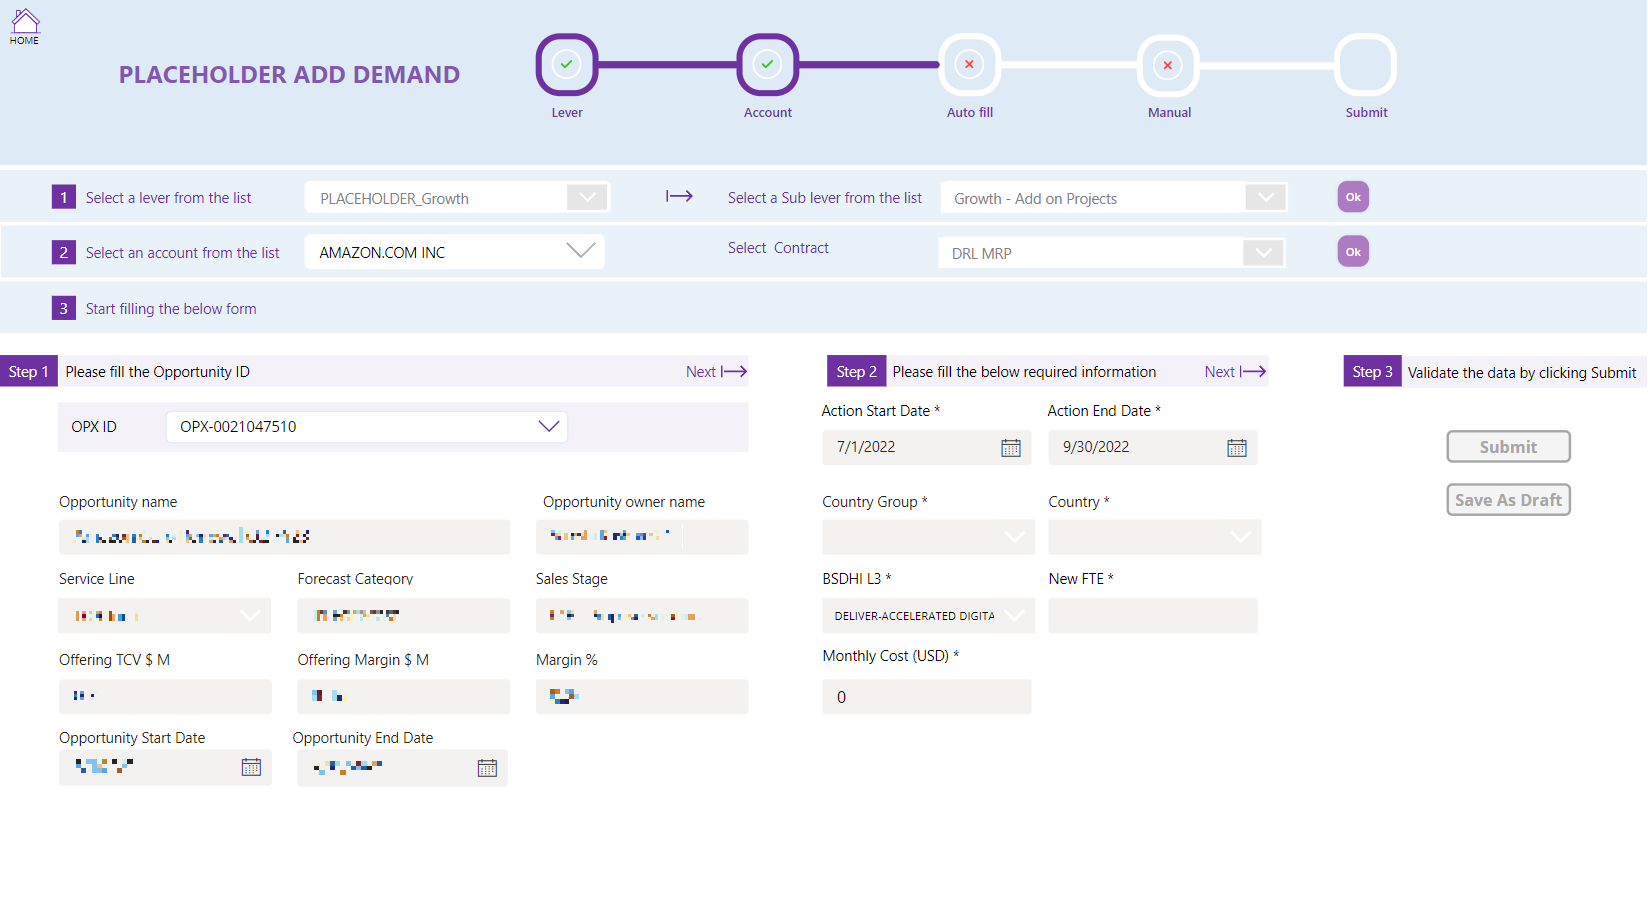
\includegraphics[scale=0.4,keepaspectratio]{Rapport de stage PFE chez DXC/figures/Placeholder_add_demand.png}
    \caption{Ajout de demande - Placeholder Add Demand}
\end{figure}

La procédure pour saisir une entrée de type "Placeholder - Add demand" est la suivante :

\begin{enumerate}
    
    \item L'utilisateur commence par sélectionner le sub-lever, qui représente la catégorie de la demande d'ajout pour un projet ou bien une croissance stratégique ou autres ensuite il doit cliquer sur le bouton ok.
    \vspace{0.1cm}
    \item Ensuite l'utilisateur doit sélectionner le compte et le contrat qu'il souhaite.
    \vspace{0.1cm}
    \item Puis apparait diffèrent champ qu'il doit remplir, pour l'étape 1 il suffit de sélectionner un OPX-ID qui représente un identificateur d'une opportunité ensuite toutes les informations sont automatiquement remplis.
    \vspace{0.1cm}
    \item La deuxième étape est saisie par l'utilisateur il doit remplir toutes les informations de la demande
    \vspace{0.1cm}
    \item Finalement l'utilisateur a deux choix soit soumettre directement ou bien la soumettre en tant que brouillon s'il n'est pas sur ou souhaite changer les informations de l'entrée dans le futur

\end{enumerate}


% ========================= Modification of demand ==============================

\section{Compte - Modification de la masse salariale}

% =================================== Run-Off / Extension =======================

\subsection{Modification de la masse salariale}

\subsubsection{Présentation de l'interface :}

L'interface suivante permit la saisi d'entré de modification de position, deux types d'entrée sont possible une entré "Run-Off" qui représente une personne qui quitte DXC ou bien un entrée "extension" qui permet d'étendre la durée de contrat d'un employé.

\subsubsection{Regle de gestion:}

Le tableau suivant represente les different regle de gestion que l'interface doit respecter :

\vspace{0.2cm}

\tikzset{ 
    table/.style={
        matrix of nodes,
        row sep=-\pgflinewidth,
        column sep=-\pgflinewidth,
        nodes={
            rectangle,
            draw=black
        },
        minimum height=1.5em,
        text depth=0.5ex,
        text height=2ex,
        nodes in empty cells,
%%
        every even row/.style={
            nodes={fill=gray!70}
        },
        column 1/.style={
            nodes={text width=10em,align=center}
        },
        column 2/.style={
            nodes={text width=24em}
        },
        column 3/.style={
            nodes={text width=5em,align=center}
        },
        row 1/.style={
            nodes={
                font=\bfseries,
                align=center,
                fill=black,
                text=white,
            }
        },
        row 2/.style={
            nodes={
                fill=black,
                text=white,
                text depth=4ex,
            }
        },
        row 3/.style={
            nodes={
                fill=white,
                text=black,
                text depth=4ex,
            }
        },
        row 4/.style={
            nodes={
                fill=black,
                text=white,
                text depth=4ex,
            }
        },
        row 5/.style={
            nodes={
                fill=white,
                text=black,
                text depth=4ex,
            }
        },
        row 6/.style={
            nodes={
                fill=black,
                text=white,,
                text depth=11ex,
            }
        },
        row 7/.style={
            nodes={
                fill=white,
                text=black,
                text depth=7ex,
            }
        }
    }
}

\begin{tikzpicture}

\matrix (first) [table,text width=6em]
{
 Regle de gestion  & Description & Type \\
 RG01 & Toutes les informations de l’étape 2 doivent être remplis & Métier \\
 RG02 & Si une information de l'étape 2 ou bien 1 est vide le bouton de soumission doit être désactiver. & Métier \\
 RG03 & La valeur du FTE doit être inférieur ou égal à l'FTE actuelle de l'employé & Métier \\
 RG04  & Le champ monthly cost n'accepte que des chiffres & Métier \\
 RG06  & Une fois l'entrée soumis tout les champs doivent etre réinitialiser puis envoyer l'utilisateur a l'interface "view submission" & IHM\\
};


\end{tikzpicture}

\subsubsection{Fonctionnement de l'interface :}

\begin{figure}[H]
    \centering
    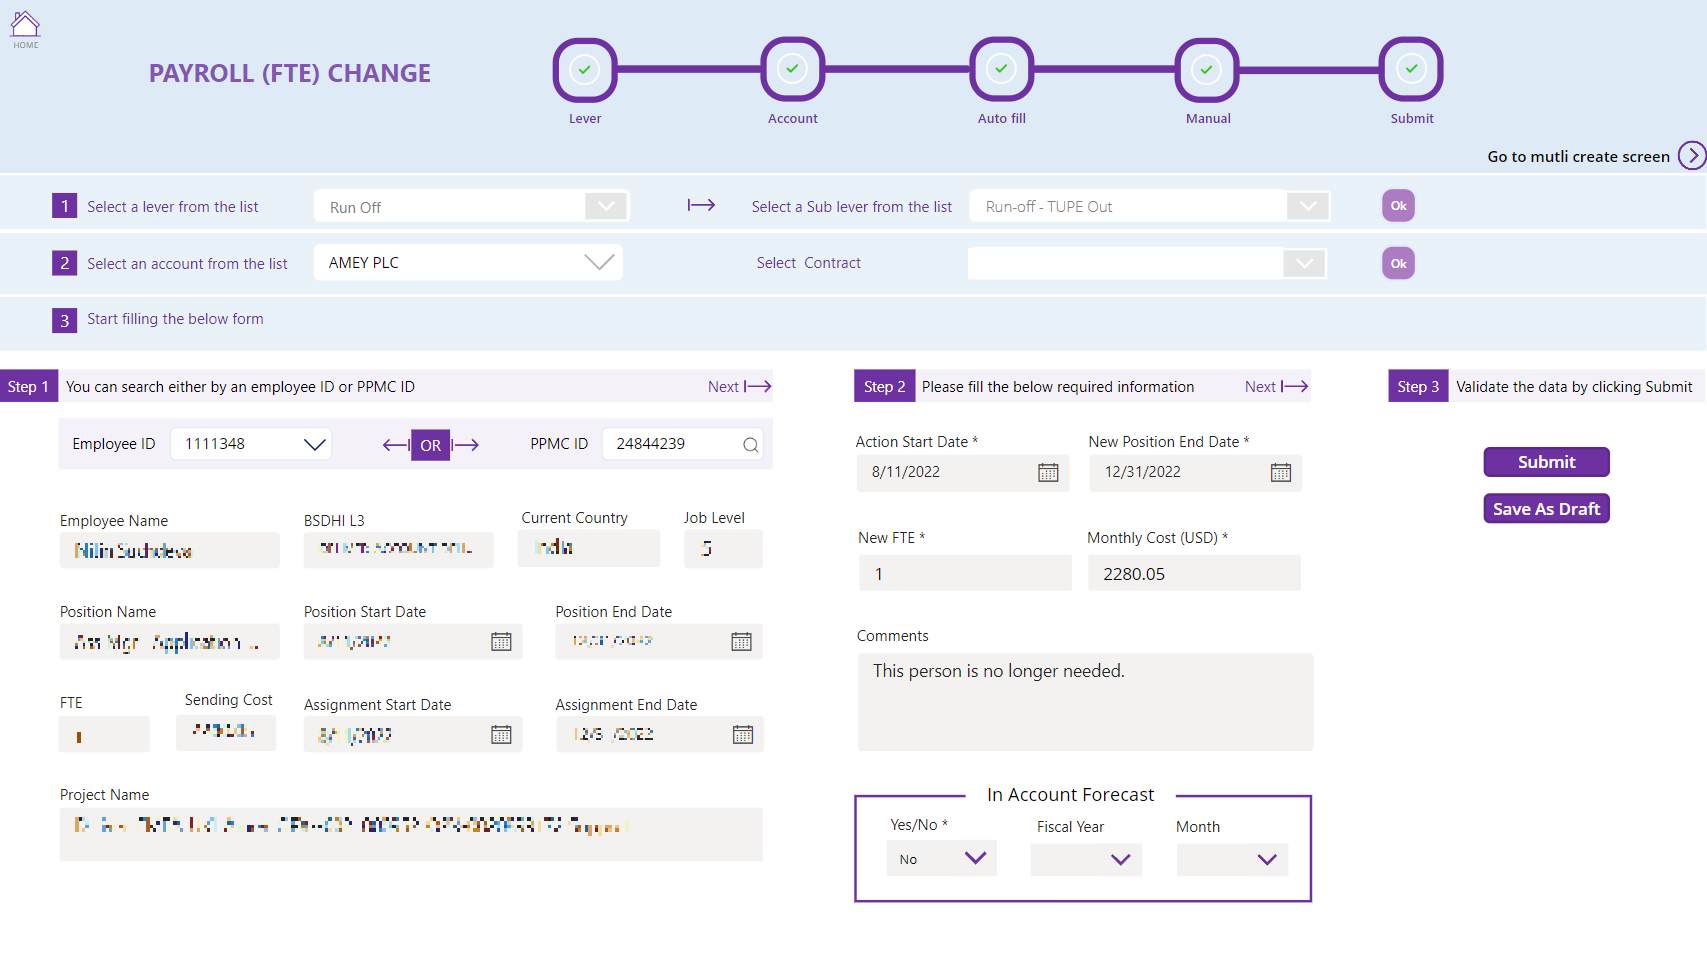
\includegraphics[scale=0.4,keepaspectratio]{Rapport de stage PFE chez DXC/figures/modification_of_demand.png}
    \caption{Compte - Modification de la masse salariale}
\end{figure}

La procédure pour saisir une entrée de type "Run Off" ou bien "Extension" est la suivante :

\begin{enumerate}
    
    \item L'utilisateur doit sélectionner le compte et le contrat qu'il souhaite.
    \vspace{0.1cm}
    \item Dans l'étape 1 l'utilisateur peut saisir un identificateur d’employée ou bien un PPMC ID pour rechercher dans la base de données est trouvé l'employé qu'il souhaite, ensuite en le sélectionnant toutes les informations sont remplis de façon automatique.
    \vspace{0.1cm}
    \item La deuxième étape est saisie par l'utilisateur il doit remplir toutes les informations pour compléter l'entrée.
    \vspace{0.1cm}
    \item Finalement l'utilisateur a deux choix soit soumettre directement ou bien la soumettre en tant que brouillon s'il n'est pas sur ou souhaite changer les informations de l'entrée dans le futur

\end{enumerate}

\newpage
Pour la saisie des entré Run-Off/ Extension, l'utilisateur est souvent amené à saisir plusieurs entré à la fois à savoir 20/30 employé ou plus qui quitte un courant poste par exemple. La saisie de ces derniers prendrait beaucoup de temps avec la manière décrite précédemment, c'est pour cela qu'une option de multi-création est présente dans cette interface. 

\vspace{0.3cm}

En cliquant sur le bouton de navigation "go to multi-create screen" l'utilisateur peut alors réaliser des soumissions en masse comme le montre la figure suivante:


\begin{figure}[H]
    \centering
    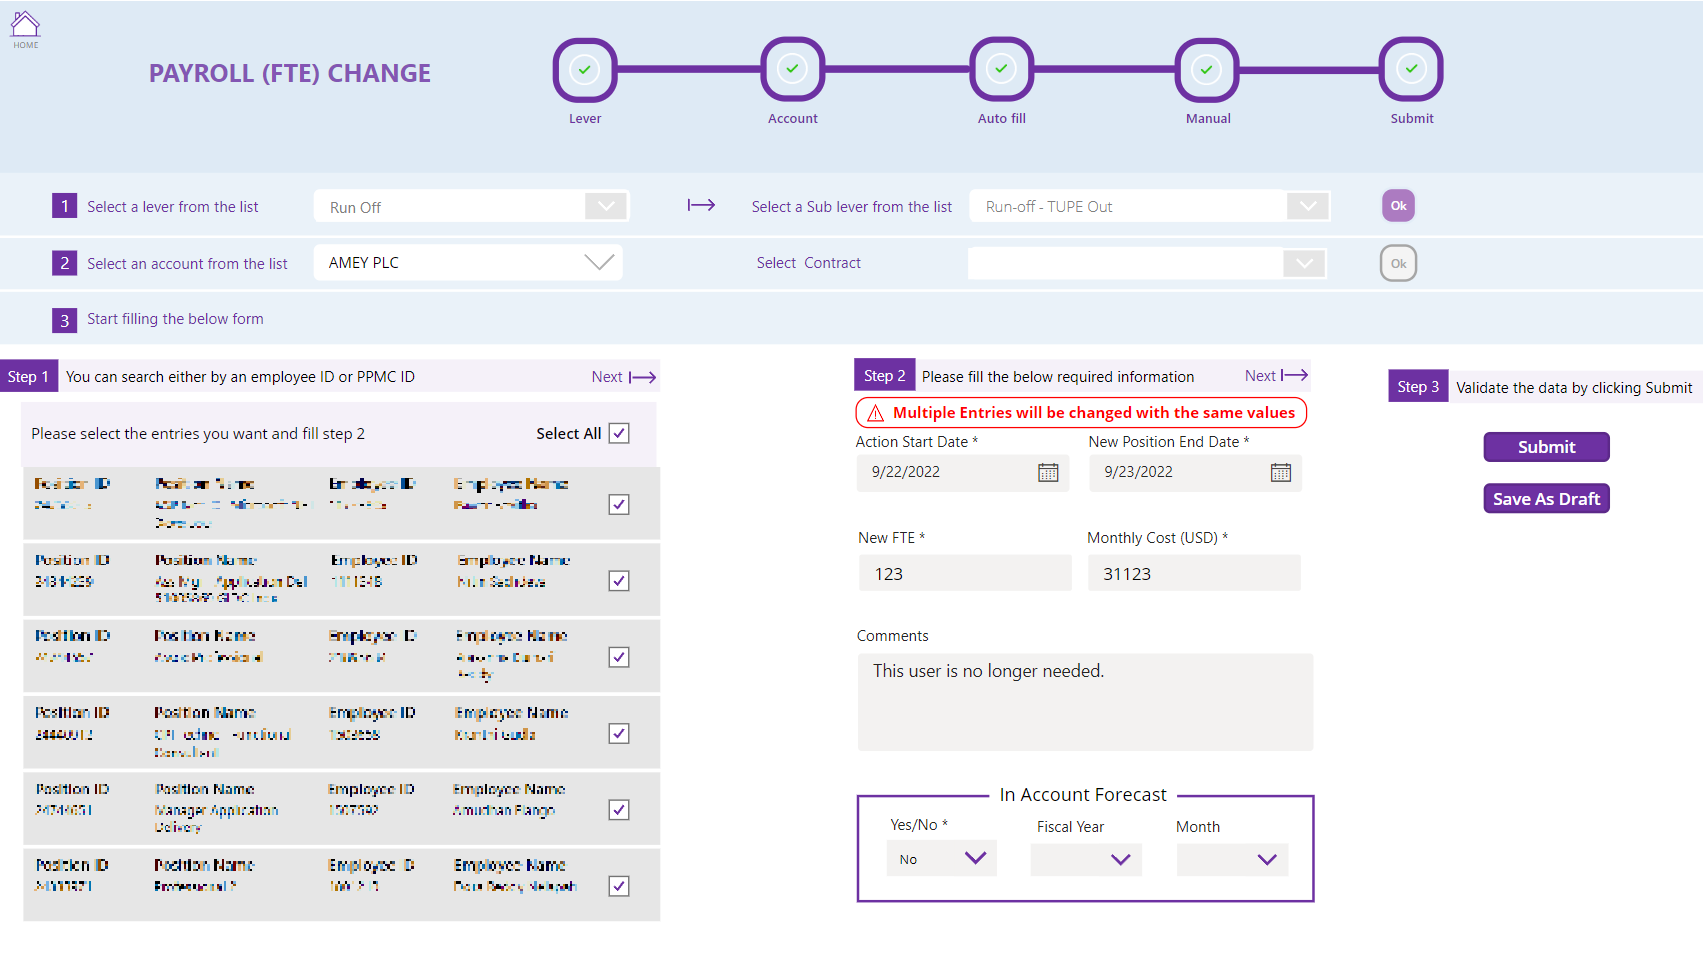
\includegraphics[scale=0.4,keepaspectratio]{Rapport de stage PFE chez DXC/figures/multi_modification_of_demand.png}
    \caption{Compte - Modification de la masse salariale en grand nombre}
\end{figure}

\begin{enumerate}
    
    \item L'utilisateur doit sélectionner le compte et le contrat qu'il souhaite.
    \vspace{0.1cm}
    \item Ensuite dans l'étape 1 il va selectionner cette fois-ci la liste des employé qu'il souhaite sasir.
    \vspace{0.1cm}
    \item Dès lors il a deux options, s’il saisit plusieurs employés ces entrée vont tous être créer avec les mêmes informations de la deuxième étape, (un message d'avertissement est montré pour guider l'utilisateur), ou bien il peut sélectionner un employé à la fois.
    \vspace{0.1cm}
    \item Finalement l'utilisateur a deux choix soit soumettre directement ou bien la soumettre en tant que brouillon s'il n'est pas sur ou souhaite changer les informations de l'entrée dans le futur
    \item L'utilisateur n'est renvoyé à l'écran "view submission" que lorsqu'il complète tous les employés sélectionnés précédemment.

\end{enumerate}


\newpage

%======================= Placeholder - Modification of demand =================================

\subsection{Placeholder Modification de la masse salariale}

\subsubsection{Présentation de l'interface :}

De la même manière que le placeholder pour l'ajout de demande, le placeholder de modification de demande permet à l'utilisateur de créer des entrées pour des future modifications.

\subsubsection{Regle de gestion:}

Le tableau suivant represente les different regle de gestion que l'interface doit respecter :

\vspace{0.2cm}

\tikzset{ 
    table/.style={
        matrix of nodes,
        row sep=-\pgflinewidth,
        column sep=-\pgflinewidth,
        nodes={
            rectangle,
            draw=black
        },
        minimum height=1.5em,
        text depth=0.5ex,
        text height=2ex,
        nodes in empty cells,
%%
        every even row/.style={
            nodes={fill=gray!70}
        },
        column 1/.style={
            nodes={text width=10em,align=center}
        },
        column 2/.style={
            nodes={text width=24em}
        },
        column 3/.style={
            nodes={text width=5em,align=center}
        },
        row 1/.style={
            nodes={
                font=\bfseries,
                align=center,
                fill=black,
                text=white,
            }
        },
        row 2/.style={
            nodes={
                fill=black,
                text=white,
                text depth=4ex,
            }
        },
        row 3/.style={
            nodes={
                fill=white,
                text=black,
                text depth=4ex,
            }
        },
        row 4/.style={
            nodes={
                fill=black,
                text=white,
                text depth=4ex,
            }
        },
        row 5/.style={
            nodes={
                fill=white,
                text=black,
                text depth=7ex,
            }
        }
    }
}

\begin{tikzpicture}

\matrix (first) [table,text width=6em]
{
 Regle de gestion  & Description & Type \\
 RG01 & Toutes les informations de l’étape 2 doivent être remplis & Métier \\
 RG02 & Si une information de l'étape 2 est vide le bouton de soumission doit être désactiver. & Métier \\
 RG03  & Le champ monthly cost n'accepte que des chiffres & Métier \\
 RG04  & Une fois l'entrée soumis tout les champs doivent etre réinitialiser puis envoyer l'utilisateur a l'interface "view submission" & IHM\\
};

\end{tikzpicture}

\subsubsection{Fonctionnement de l'interface :}

\begin{figure}[hbt!]
    \centering
    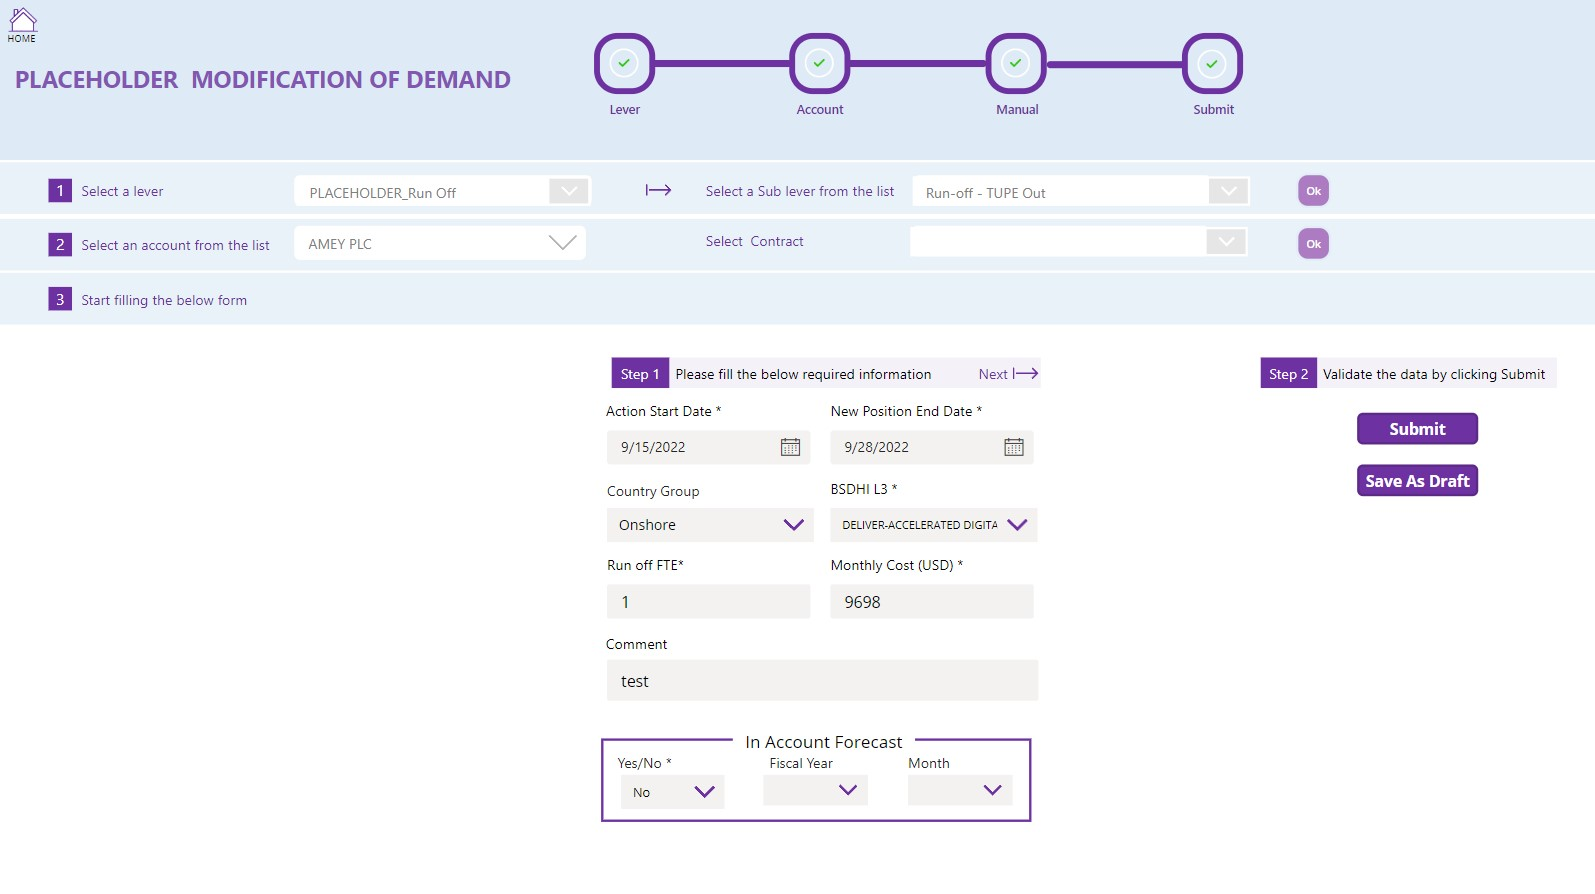
\includegraphics[scale=0.37,keepaspectratio]{Rapport de stage PFE chez DXC/figures/placeholder_modification_of_demand.jpg}
    \caption{Placeholder - Modification de la masse salariale}
\end{figure}

La procédure pour saisir une entrée de type "Placeholder - Modification of demand" est la suivante :

\begin{enumerate}
    
    \item L'utilisateur doit sélectionner le compte et le contrat qu'il souhaite.
    \vspace{0.1cm}
    \item Il doit ensuite remplir les informations de l'étape 1.(Puisque ce Placeholder n'est qu'une sorte de préparation pour une future entrée de modification l'utilisateur ne sélectionne pas un employé spécifique)
    \vspace{0.1cm}
    \item Finalement l'utilisateur a deux choix soit soumettre directement ou bien la soumettre en tant que brouillon s'il n'est pas sur ou souhaite changer les informations de l'entrée dans le futur

\end{enumerate}

%======================================== Account View submission ===============================

\section{Compte - Consultation des soumissions}

\subsubsection{Présentation de l'interface :}

Le module de consultation des soumissions permet à l'utilisateur de consulter ces soumissions plusieurs filtre sont présent pour faciliter la recherche, L'utilisateur peut aussi modifier, dupliquer, créer une entrée DCT à travers cette interface.

\subsubsection{Regle de gestion:}

Le tableau suivant represente les different regle de gestion que l'interface doit respecter :

\vspace{0.2cm}

\tikzset{ 
    table/.style={
        matrix of nodes,
        row sep=-\pgflinewidth,
        column sep=-\pgflinewidth,
        nodes={
            rectangle,
            draw=black
        },
        minimum height=1.5em,
        text depth=0.5ex,
        text height=2ex,
        nodes in empty cells,
%%
        every even row/.style={
            nodes={fill=gray!70}
        },
        column 1/.style={
            nodes={text width=10em,align=center}
        },
        column 2/.style={
            nodes={text width=24em}
        },
        column 3/.style={
            nodes={text width=5em,align=center}
        },
        row 1/.style={
            nodes={
                font=\bfseries,
                align=center,
                fill=black,
                text=white,
            }
        },
        row 2/.style={
            nodes={
                fill=black,
                text=white,
                text depth=4ex,
            }
        },
        row 3/.style={
            nodes={
                fill=white,
                text=black,
                text depth=4ex,
            }
        },
        row 4/.style={
            nodes={
                fill=black,
                text=white,
                text depth=4ex,
            }
        },
        row 5/.style={
            nodes={
                fill=white,
                text=black,
                text depth=7ex,
            }
        }
    }
}

\begin{tikzpicture}

\matrix (first) [table,text width=6em]
{
 Regle de gestion  & Description & Type \\
 RG01 & L’utilisateur doit pouvoir combiner plusieurs filtres à la fois & Métier \\
 RG02 & Le filtre "My Entries" doit être active par défaut lors de l’accès a l'interface & Métier \\
 RG03  & En cliquant sur une entrée l'utilisateur doit voir un menu latéral qui lui permet de modifier dupliquer ou créer un DCT à partir d'une entrée. & Métier \\
 RG04  & Si une entrée est modifiée l'utilisateur doit pouvoir voir le changement instantanément dans la table des données & Métier\\
};

\end{tikzpicture}

\subsubsection{Fonctionnement de l'interface :}

\begin{figure}[H]
    \centering
    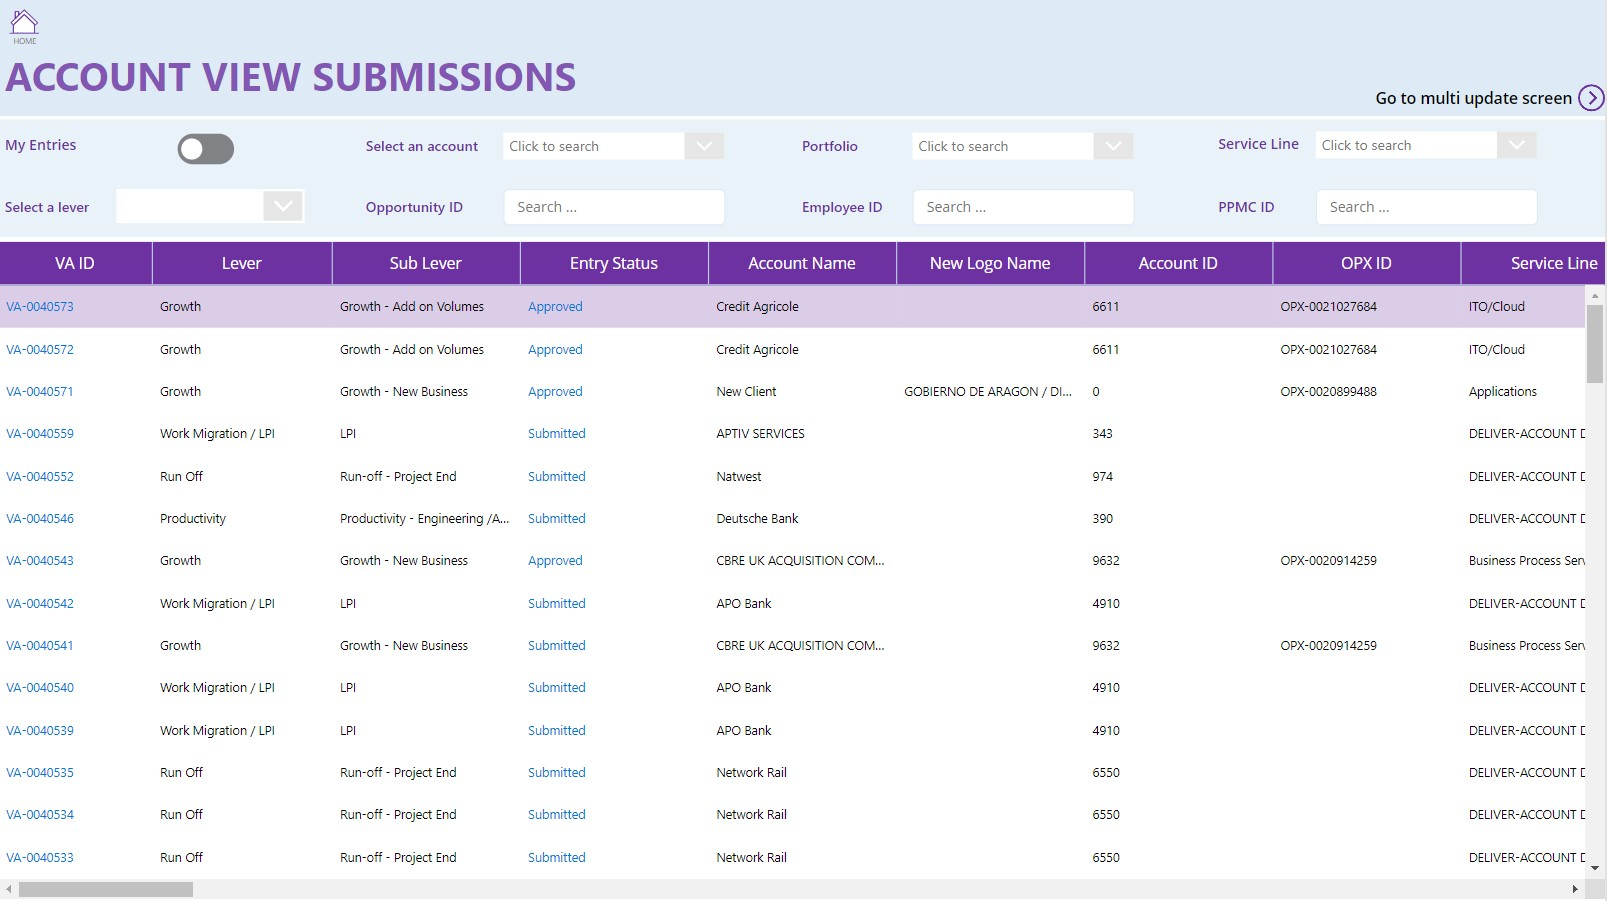
\includegraphics[scale=0.4,keepaspectratio]{Rapport de stage PFE chez DXC/figures/view_submission.jpg}
    \caption{Compte - Consultation des soumissions}
\end{figure}

\begin{enumerate}
    
    \item L'utilisateur peut par défaut ne voir que les entrée qui lui appartienne
    \vspace{0.1cm}
    \item Il peut ensuite filtrer les données en utilisant les different filtre.
    \vspace{0.1cm}
    \item En cliquant sur une entré un menu latérale apparait selon le type de l'entrée

\end{enumerate}

Si l'entrée n'est pas de type placeholder l'utilisateur est renvoyé a ce menu : 

\begin{figure}[H]
    \centering
    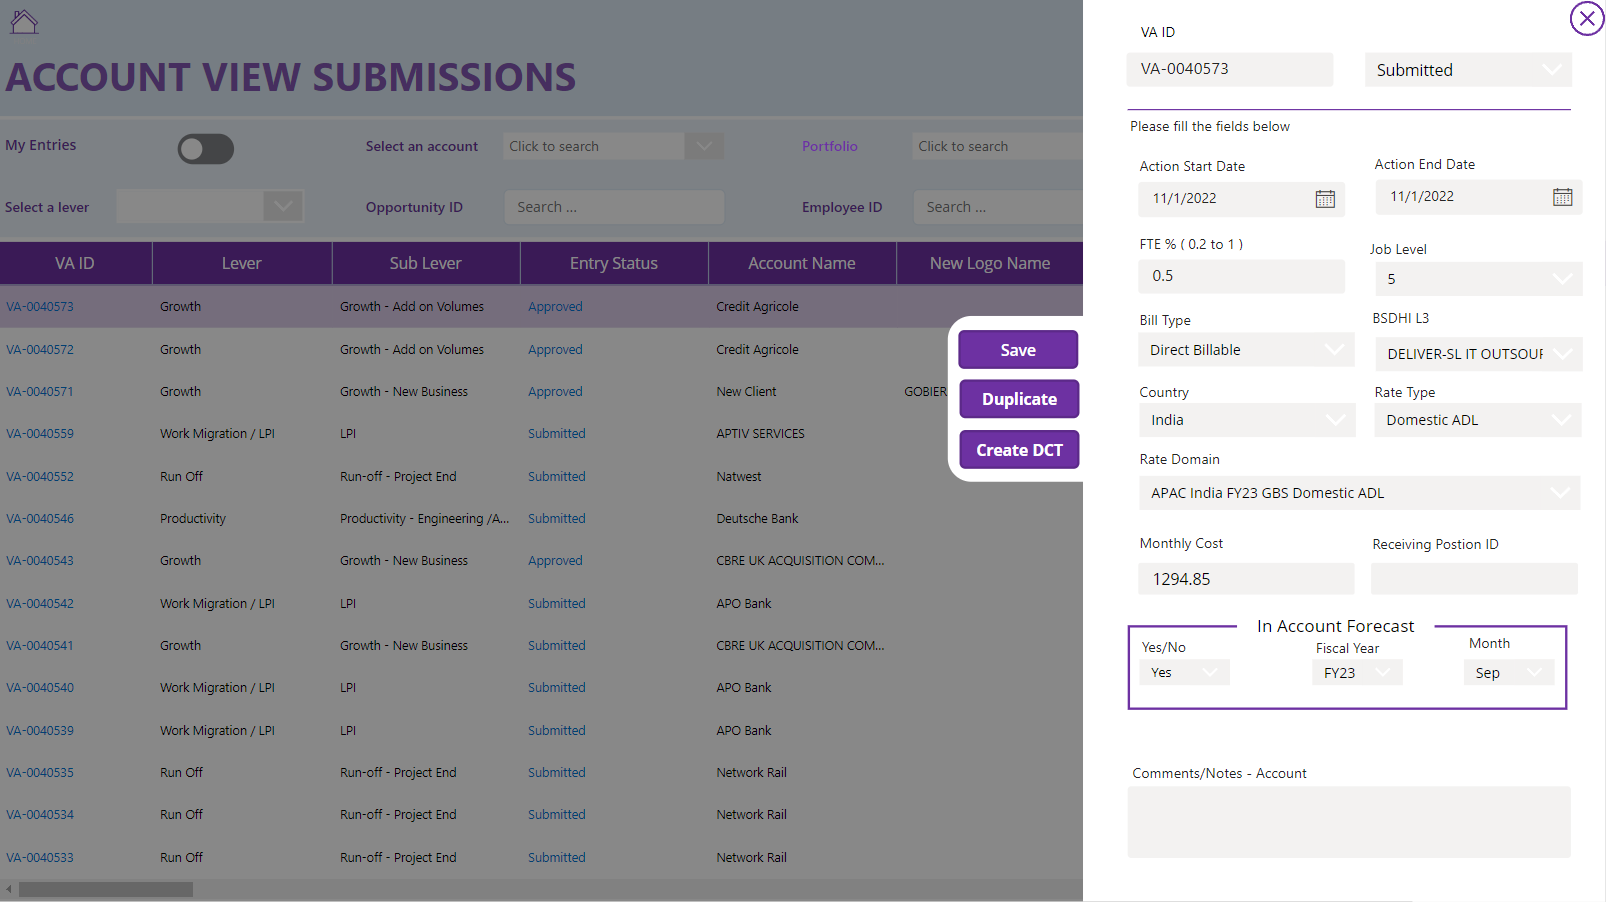
\includegraphics[width=16cm, height=7cm]{Rapport de stage PFE chez DXC/figures/account_view_side_menu.png}
    \caption{Compte - Consultation des soumissions - Menu latéral}
\end{figure}

\begin{enumerate}
    
    \item L'utilisateur peut alors modifier les information est cliquer sur le bouton "save" pour enregistrer ces modifications
    \vspace{0.1cm}
    \item L'utilisateur peut dupliquer cette entrée en cliquant sur le bouton "Duplicate"
    \vspace{0.1cm}
    \item L'utilisateur peut aussi créer une entré DCT à travers cette entrée
    \item Si l'utilisateur souhaite annuler il n'a qu'à cliquer sur la croix en haut à droite.

\end{enumerate}

Il existe aussi une option pour effectuer une modification en masse des entrées pour cela l'utilisateur doit cliquer sur le bouton "Go to multi update screen", il est renvoyé vers l'interface suivante:

\begin{figure}[H]
    \centering
    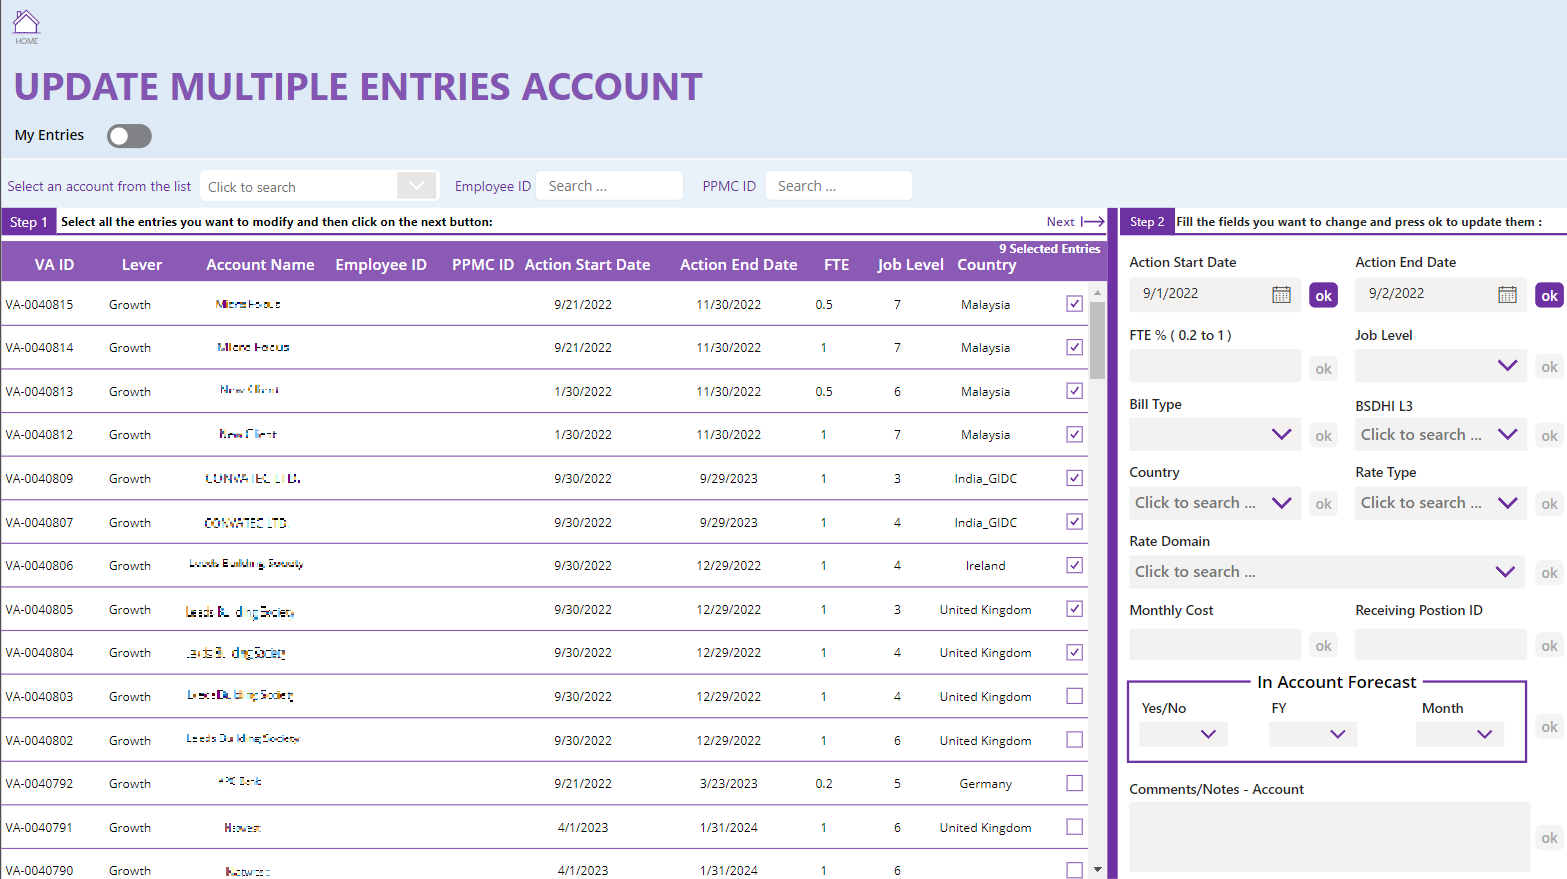
\includegraphics[scale=0.4,keepaspectratio]{Rapport de stage PFE chez DXC/figures/multi_update_view_submission.png}
    \caption{Compte - Consultation des soumissions}
\end{figure}

\begin{enumerate}
    
    \item L'utilisateur sélectionne les différentes entrées qu'il souhaite modifier et puis clique sur le bouton next.
    \vspace{0.1cm}
    \item Ensuite l'utilisateur est présenté avec les différents champs qu'il peut modifier.
    \vspace{0.1cm}
    \item L'utilisateur doit saisir la valeur du champ qu'il veut modifier, ensuite cliquer sur le bouton ok, cela va modifier cette valeur pour toutes les entrées sélectionner
    \vspace{0.1cm}
    \item Une fois cliquer sur le buton ok ce dernier va réinitialiser le champ et ce désactiver.

\end{enumerate}

% ============================ DCT Position Management =======================

\section{DCT Position Level Management}

% ============================ DCT Position Management =======================

\subsection{DCT Position Level Management - Creation de demande}

\subsubsection{Présentation de l'interface :}

DCT est l'acronyme de Demand creation template, après avoir créer une entrée de type VA est confirmer cette dernière, une entré DCT va être créer pour compléter le processus.

\subsubsection{Regle de gestion:}

Le tableau suivant represente les different regle de gestion que l'interface doit respecter :

\vspace{0.2cm}

\tikzset{ 
    table/.style={
        matrix of nodes,
        row sep=-\pgflinewidth,
        column sep=-\pgflinewidth,
        nodes={
            rectangle,
            draw=black
        },
        minimum height=1.5em,
        text depth=0.5ex,
        text height=2ex,
        nodes in empty cells,
%%
        every even row/.style={
            nodes={fill=gray!70}
        },
        column 1/.style={
            nodes={text width=10em,align=center}
        },
        column 2/.style={
            nodes={text width=24em}
        },
        column 3/.style={
            nodes={text width=5em,align=center}
        },
        row 1/.style={
            nodes={
                font=\bfseries,
                align=center,
                fill=black,
                text=white,
            }
        },
        row 2/.style={
            nodes={
                fill=black,
                text=white,
                text depth=22ex,
            }
        },
        row 3/.style={
            nodes={
                fill=white,
                text=black,
                text depth=4ex,
            }
        },
        row 4/.style={
            nodes={
                fill=black,
                text=white,
                text depth=4ex,
            }
        },
        row 5/.style={
            nodes={
                fill=white,
                text=black,
                text depth=7ex,
            }
        },
        row 6/.style={
            nodes={
                fill=white,
                text=black,
                text depth=5ex,
            }
        },
        row 7/.style={
            nodes={
                fill=white,
                text=black,
                text depth=5ex,
            }
        },
        row 8/.style={
            nodes={
                fill=white,
                text=black,
                text depth=7ex,
            }
        }
    }
}

\begin{tikzpicture}

\matrix (first) [table,text width=8em]
{
 Regle de gestion  & Description & Type \\
 RG01 & Les champs suivant sont obligatoires: Financial client Name, DCT Type, OPX-ID, Project ID, Project Sold, Early staffing, Bill Type, Monthly position cost,Monthly Position Revenue, Reason Position Needed, Start Date/end Date/FTE, Country, Location Contractually Constraint, Position Work Location, Level Required, Resource Type, Requested Ressource & Métier \\
 RG02 & Si un champ obligatoire est vide le bouton de soumission doit être désactiver & Métier \\
 RG03 & Si un utilisateur  saisit un OPX-ID et clique sur la loupe le Financial client name doit être  automatiquement saisit & Métier \\
 RG04 & Si l'utilisateur saisie un "Requested Ressource" le "Ressource Pool" doit etre automatiquement remplis & Métier\\
 RG05 & Monthly Position Cost et revenue n'accepte que des chiffres & Métier\\
 RG06 & Si le DCT Type est un Addon New les champs Project Sold et early staffing sont désactiver & Métier\\
 RG07 & Une fois l'entrée soumis tout les champs doivent etre réinitialiser puis envoyer l'utilisateur a l'interface "DCT View Submission" & IHM\\
};

\end{tikzpicture}

\subsubsection{Fonctionnement de l'interface :}

\begin{figure}[H]
    \centering
    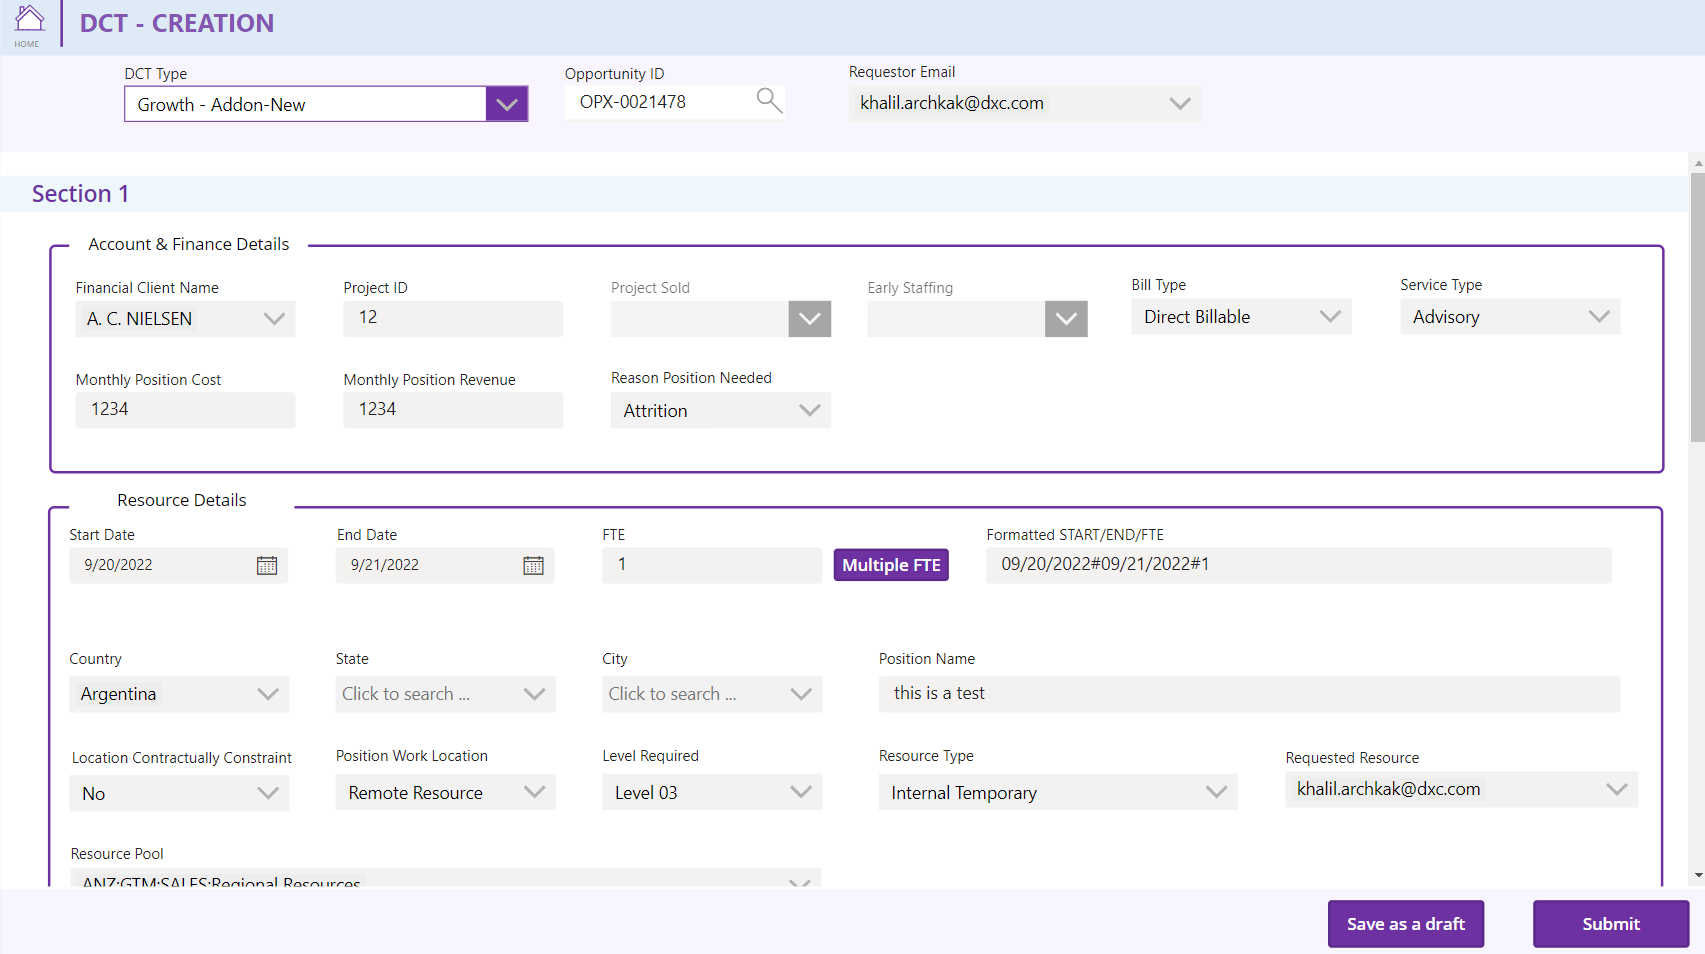
\includegraphics[scale=0.4,keepaspectratio]{Rapport de stage PFE chez DXC/figures/DCT_Create.png}
    \caption{DCT Position Level Management - Creation de demande }
\end{figure}

La procédure pour saisir une entrée de type "DCT - Creation" est la suivante :

\begin{enumerate}
    
    \item L'utilisateur doit d'abord sélectionner le type de DCT qu'il veut créer.
    \vspace{0.1cm}
    \item Ensuite il doit remplir tous les champs obligatoires.
    \vspace{0.1cm}
    \item Et finalement deux options s’offrent à lui soit directement soumettre son entrée ou bien l'enregistrer en tant que brouillon s'il n'est pas sur des informations et souhaite les modifier dans le futur.

\end{enumerate}

% ================== DCT Position management - UPDATE =========================

\subsection{DCT Position Level Management - Mise a jour de la demande}

\subsubsection{Présentation de l'interface :}

Cette interface permet de saisire une modification au niveau d'un DCT, il a le meme principe que le precedent : 

\subsubsection{Regle de gestion:}

Le meme tableau de regle de gestion vu précedement est utilisée poru cette interface

\subsubsection{Fonctionnement de l'interface :}

\begin{figure}[H]
    \centering
    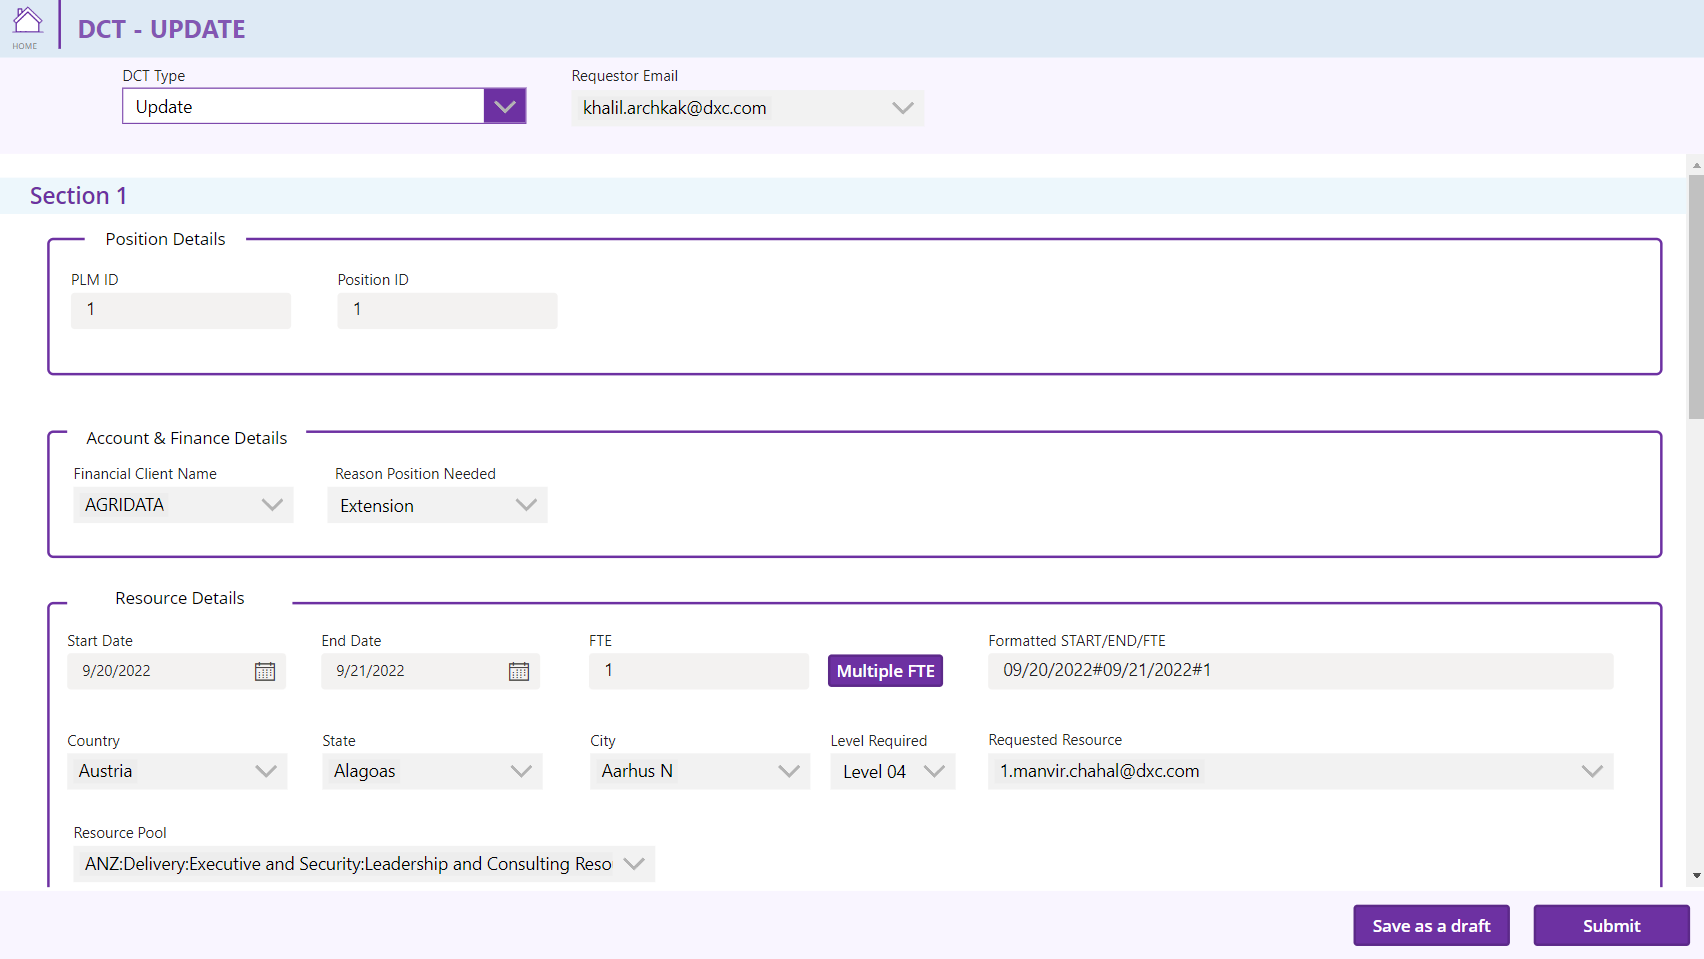
\includegraphics[scale=0.4,keepaspectratio]{Rapport de stage PFE chez DXC/figures/DCT_Update.png}
    \caption{DCT Position Level Management - Mise a jour de la demande}
\end{figure}

L'interface est à peu près la même que la précédente, la seule différence est dans la position des champs, dans ce dernier le premier champ à modifier est le "PLM ID" ainsi que le "Position ID", la procédure de saisie d'une demande de modification est la suivante :

\begin{enumerate}
    
    \item L'utilisateur doit d'abord sélectionner le type de DCT qu'il veut créer.
    \vspace{0.1cm}
    \item L'utilisateur ne doit saisir que les champs obligatoires selon le type du DCT.
    \vspace{0.1cm}
    \item Et finalement deux options s’offrent à lui soit directement soumettre son entrée ou bien l'enregistrer en tant que brouillon s'il n'est pas sur des informations et souhaite les modifier dans le futur.

\end{enumerate}

% ================================ DCT View submission ===============================
\subsection{DCT Position Level Management - Consultation des soumissions}

\subsubsection{Présentation de l'interface :}

Cette interface permet de consulter ses soumissions, et propose aussi la possibilité de modifier, dupliquer, annuler ou bien attacher un mail d'approbation avec la demande.

\subsubsection{Regle de gestion:}

Le tableau suivant represente les different regle de gestion que l'interface doit respecter :

\vspace{0.2cm}

\tikzset{ 
    table/.style={
        matrix of nodes,
        row sep=-\pgflinewidth,
        column sep=-\pgflinewidth,
        nodes={
            rectangle,
            draw=black
        },
        minimum height=1.5em,
        text depth=0.5ex,
        text height=2ex,
        nodes in empty cells,
%%
        every even row/.style={
            nodes={fill=gray!70}
        },
        column 1/.style={
            nodes={text width=10em,align=center}
        },
        column 2/.style={
            nodes={text width=24em}
        },
        column 3/.style={
            nodes={text width=5em,align=center}
        },
        row 1/.style={
            nodes={
                font=\bfseries,
                align=center,
                fill=black,
                text=white,
            }
        },
        row 2/.style={
            nodes={
                fill=black,
                text=white,
                text depth=2ex,
            }
        },
        row 3/.style={
            nodes={
                fill=white,
                text=black,
                text depth=4ex,
            }
        },
        row 4/.style={
            nodes={
                fill=black,
                text=white,
                text depth=4ex,
            }
        },
        row 5/.style={
            nodes={
                fill=white,
                text=black,
                text depth=5ex,
            }
        }
    }
}

\begin{tikzpicture}

\matrix (first) [table,text width=8em]
{
 Regle de gestion  & Description & Type \\
 RG01 & Le bouton "My entries" doit etre activer par défaut & Métier \\
 RG02 & Les entrées doivent être trié selon l'ordre de création, dans l'ordre croissant. & Métier \\
 RG03 & Les bouton "cancel submission" et "edit" ne sont active que lorsque l'entrée et dans le statut "draft" ou bien "review" & Métier \\
 RG04 & Le bouton attach approval n'est active que l'orsque l'utilisateur ajoute un fichier & Métier\\
};

\end{tikzpicture}

\subsubsection{Fonctionnement de l'interface :}

Aprés avoir saisit l'entrée l'utilisateur est envoyé vers l'interface de consultation des soumissions:

\begin{figure}[H]
    \centering
    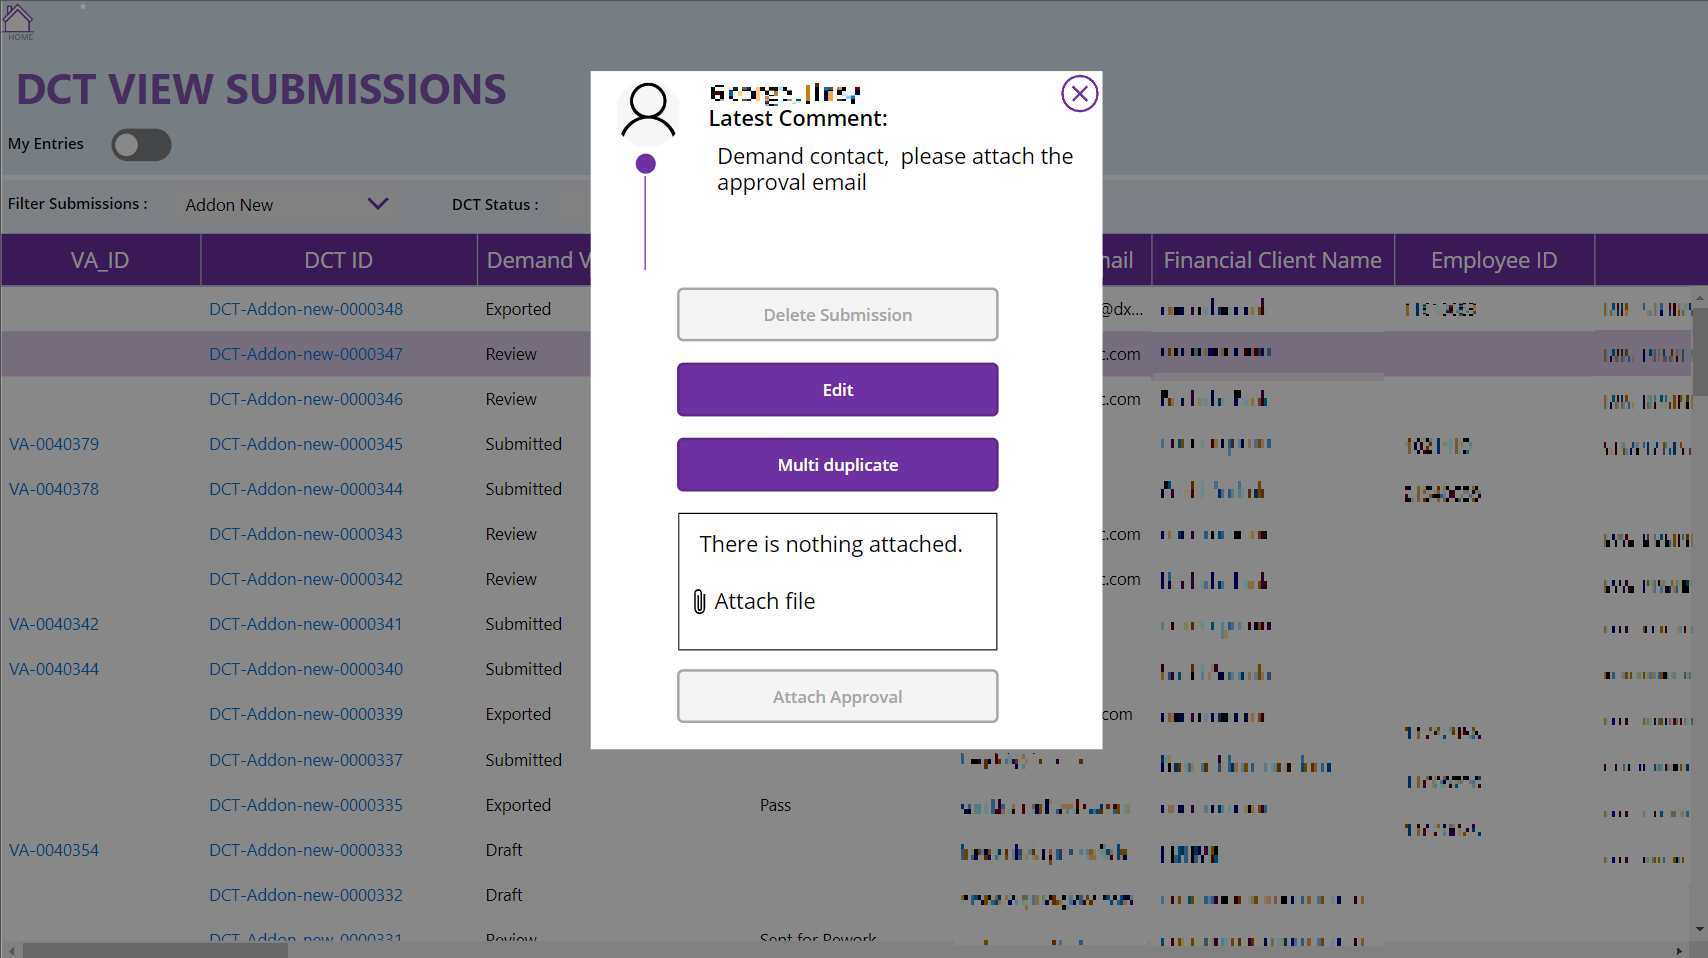
\includegraphics[scale=0.4,keepaspectratio]{Rapport de stage PFE chez DXC/figures/DCT_view_submission.png}
    \caption{DCT Position Level Management - Consultation des soumissions}
\end{figure}

L'interface est à peu près la même que la précédente, la seule différence est dans la position des champs, dans ce dernier le premier champ à modifier est le "PLM ID" ainsi que le "Position ID", la procédure de saisie d'une demande de modification est la suivante :

\begin{enumerate}
    
    \item L'utilisateur peut consulter les informations de sont entrée en parcourant le tableau, il peut aussi filter selon le status de l'entrée
    \vspace{0.1cm}
    \item En cliquant sur l'entrée un menu se presente a l'utilisateur
    \vspace{0.1cm}
    \item S’il souhaite annuler l'entrée, il suffit de cliquer sur le bouton "cancel submission" ce dernier l'envoie vers un autre menu de confirmation et puis il peut annuler son entrée.
    \vspace{0.1cm}
    \item S’il souhaite modifier son entrée il suffit de cliquer sur le bouton "Edit" l'utilisateur est alors renvoyé vers le formulaire avec toutes les informations préremplie il suffit alors de modifier son entrée puis resoumettre.
    \vspace{0.1cm}
    \item En cliquant sur le bouton "Multi duplicate" l'utilisateur peut dupliquer son entrée autant de fois qu'il le souhaite.
    \vspace{0.1cm}
    \item Si l'entrée nécessite un mail d'approbation de la part de L'ADL ou autre l'utilisateur peut alors soumettre ce fichier en cliquant sur le bouton "Attach Approval".

\end{enumerate}

% ======================= DCT Demand validation checks =============================

\subsection{DCT Position Level Management - Validation des entrée}

\subsubsection{Présentation de l'interface :}

Cette interface permet de valider les soumission DCT saisit par les comptes.

\subsubsection{Regle de gestion:}

Le tableau suivant represente les different regle de gestion que l'interface doit respecter :

\vspace{0.2cm}

\tikzset{ 
    table/.style={
        matrix of nodes,
        row sep=-\pgflinewidth,
        column sep=-\pgflinewidth,
        nodes={
            rectangle,
            draw=black
        },
        minimum height=1.5em,
        text depth=0.5ex,
        text height=2ex,
        nodes in empty cells,
%%
        every even row/.style={
            nodes={fill=gray!70}
        },
        column 1/.style={
            nodes={text width=10em,align=center}
        },
        column 2/.style={
            nodes={text width=24em}
        },
        column 3/.style={
            nodes={text width=5em,align=center}
        },
        row 1/.style={
            nodes={
                font=\bfseries,
                align=center,
                fill=black,
                text=white,
            }
        },
        row 2/.style={
            nodes={
                fill=black,
                text=white,
                text depth=2ex,
            }
        },
        row 3/.style={
            nodes={
                fill=white,
                text=black,
                text depth=6ex,
            }
        },
        row 4/.style={
            nodes={
                fill=black,
                text=white,
                text depth=8ex,
            }
        },
        row 5/.style={
            nodes={
                fill=white,
                text=black,
                text depth=9ex,
            }
        },
        row 6/.style={
            nodes={
                fill=white,
                text=black,
                text depth=8ex,
            }
        },
        row 7/.style={
            nodes={
                fill=white,
                text=black,
                text depth=5ex,
            }
        }
    }
}

\begin{tikzpicture}

\matrix (first) [table,text width=8em]
{
 Regle de gestion  & Description & Type \\
 RG01 & Le bouton "My entries" doit être active par défaut. & Métier \\
 RG02 & Les entrées ne doivent être visible que lorsque le statut et "Submitted" ou bien "Assigned". & Métier \\
 RG03 & L'utilisateur peut prendre la possession d'une entrée, cette dernière sera verrouiller pour tous les autres utilisateurs & Métier \\
 RG04 & Si l'utilisateur prend possession d'une entrée, son statut se modifie est devient "Assigned", le champ ownership est aussi remplis avec l'email de l'utilisateur. & Métier\\
 RG05 & Si l'utilisateur clique sur le bouton "submit" cette entrée est définitivement verrouiller ne peut plus être modifier. & Métier\\
 RG06 & Si l'utilisateur soumet son entrée, cette dernière est verrouillée et ne peut plus être modifier. & Métier\\
};

\end{tikzpicture}

\subsubsection{Fonctionnement de l'interface :}

\begin{figure}[H]
    \centering
    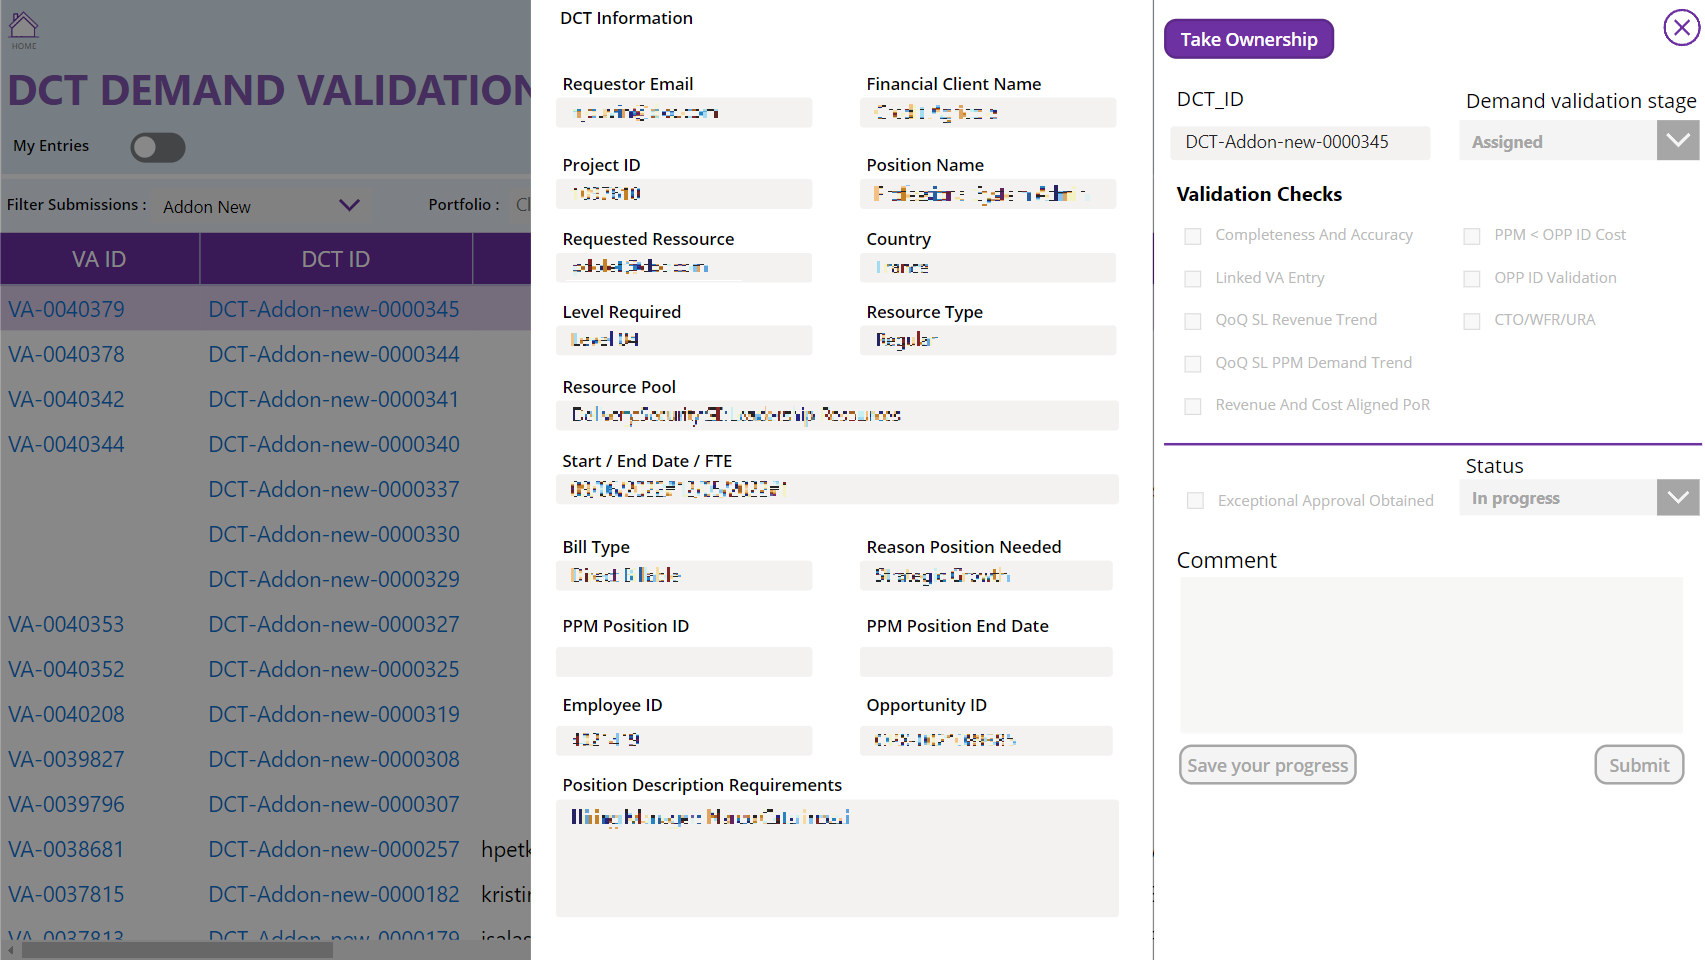
\includegraphics[scale=0.4,keepaspectratio]{Rapport de stage PFE chez DXC/figures/DCT_demand_validation_checks.png}
    \caption{DCT Position Level Management - Validation des entrée}
\end{figure}

La procedure pour valider une entrée est la suivante:

\begin{enumerate}
    
    \item L'utilisateur peut filtrer les soumissions selon le "portfolio" ou bien le nom du client pour faciliter la recherche.
    \vspace{0.1cm}
    \item En cliquant sur l'entrée un menu latérale se présente à l'utilisateur.
    \vspace{0.1cm}
    \item L'utilisateur doit d'abord prendre la possession de l'entrée pour pouvoir commencer le processus de validation.
    \vspace{0.1cm}
    \item Il va ensuite vérifier les différentes informations et cocher les vérification valides.
    \vspace{0.1cm}
    \item Si l'entrée n'est pas complète ce dernier peut la renvoyer avec un commentaire ainsi et un statut review pour être complété par le responsable du compte.
    \vspace{0.1cm}
    \item Deux options s'offre à l'utilisateur soit sauvegarder sa progression ou bien soumettre l'entrée lors de la fin du processus de validation.

\end{enumerate}

\section{Conclusion}
Dans ce chapitre nous avons présenté les principales interfaces de l'application ainsi que leurs règles de gestion et fonctionnement.